\chapter{First-order reversal curve diagram modelling of framboidal greigite}
\label{ch:res-4}

\section*{Abstract}
In this chapter...\par

\section{Introduction}
Introduction goes here...\par

\section{Methodology}
\subsection{The micromagnetic method}
A ferromagnetic (in the broad sense, i.e., including ferrimagnetic behaviour) material has a Gibbs free-energy functional (excluding the effects of thermal fluctuations and magnetostriction) which can be written as \citep{Brown}:
\begin{equation}
E_\text{G} = \int_{\Omega} (\phi_{\text{exchange}} + \phi_{\text{anisotropy}} + \phi_{\text{stray}} + \phi_{\text{external}})\,\text{d}^3 \boldsymbol{r},
\end{equation}
where $\Omega$ is the ferromagnetic volume and $\text{d}^3 \boldsymbol{r}$ the volume differential, so integrations is carried out over the ferromagnetic body. Here,
\begin{equation}
\phi_{\text{exchange}}=A|\nabla\boldsymbol{m}|^2,
\end{equation}
where $\boldsymbol{m}$ is the reduced (unitary) magnetisation vector and $A$ the exchange stiffness constant, is an expression providing a continuum approximation of the energy density due to quantum-mechanical exchange forces between atomic spins \citep{Landau1935}.
\begin{equation}
\phi_{\text{anisotropy}}=\frac{K_1}{2}\sum_{i\neq j}\gamma_i^2\gamma_j^2 + K_2\prod_i\gamma_i^2,
\end{equation}
where $\gamma_i$ denote the direction cosines and $K_1,K_2$ the first and second magnetocrystalline (MCA) anisotropy constants, respectively, is the MCA energy density for cubic-anisotropic ferromagnets. In terms of the reduced magnetisation vector components this has the form:
\begin{equation}
\phi_{\text{anisotropy}}=K_1(m_x^2m_y^2+m_y^2m_z^2+m_z^2m_x^2),
\end{equation}
where $K_2$ has been neglected since in the cubic anisotropy system we are assuming, $K_1$ is the dominant term at room temperature. The magnetic Gibbs free-energy associated with the magnetostatic self-interaction of the ferromagnetic body and the stray magnetic field $\boldsymbol{H}_{\text{stray}}$ it produces is given by:
\begin{equation}
\phi_{\text{stray}}=-\frac{\mu_0M_\text{S}}{2} \boldsymbol{m} \cdot \boldsymbol{H}_{\text{stray}}
\end{equation}
where $M_\text{S}$ is the saturation magnetisation and $\mu_0=4\pi \times 10^{{-}7}\,\text{T}\text{m}/\text{A}$ is the magnetic constant or vacuum permeability. Finally, the energy density due to the magnetostatic interaction of the ferromagnetic body and an external field $\boldsymbol{H}_{\text{external}}$ is:
\begin{equation}
\phi_{\text{external}}=-\mu_0 M_{\text{S}} \boldsymbol{m} \cdot \boldsymbol{H}_{\text{external}}.
\end{equation}

From thermodynamics, it is well known that under isothermal and isobaric conditions a system will be driven spontanteously toward an equilibrium state with locally minimal Gibbs free-energy. Micromagnetic algorithms aim to find the equilibrium magnetisation $\boldsymbol{m}$ by minimising the Gibbs free-energy functional \citep{Fischbacher2017}. Here, a modified gradient-descent method \citep{OConbhui2017} is used for this endeavour.\par

Numerical solutions require a discretisation of the spatial domain into a grid or \textit{mesh} with a finite number of points on which numerical solutions are calculated. In FEMs, three-dimensional space is decomposed into tetrahedral pieces called finite elements with the vertices of these elements called the nodes. On each of the mesh nodes, a unit vector is initially defined to create an initial guess; the micromagnetic algorithm then attempts to minimise the magnetic Gibbs free-energy by variating the orientation of each of these vectors while ensuring they remain unitary. In micromagnetic theory \citep{Brown} there are some linearisations, which means that there should not be large variations in the direction of $\boldsymbol{m}$ between neigbouring nodes. For unconstrained micromagnetic models it is expected that the microstructure will contain nouniform structures at least to some degree. To model nonuniform structures it is sufficient that the spatial discretisation in the model is always smaller than the exchange length $l_\text{exch} = \sqrt{2A/\mu_0M_\text{S}^2}$ \citep{Rave1998}, which for greigite is $l_\text{exch} \approx 6.6\, \text{nm}$; a maximum element size of 5$\nm$ has been chosen for all the meshes. The non-local problem of calculating the stray field is handled via a hybrid finite-element/boundary-element formulation \citep{Fredkin1990}.\par

\subsection{The FORC model}
Ferromagnetic materials have magnetisation states that are dependent on their magnetic (or thermal, chemical) history. This is the well-known phenomenon of magnetic hysteresis \citep{Mayergoyz1986}. Standard hysteresis measurements proceed by saturating the magnetisation by applying a saturating magnetic field $\boldsymbol{B}=\mu_0\boldsymbol{H}$ with strength $B_{\text{sat}}$; in this saturated state, magnetisations are uniform and completely aligned with the applied field. Gradually, the magnetic field strength is decreased to desaturate the magnetic material. A curve $M=M(B)$ of the material's scalar magnetisation $M=\boldsymbol{M}\cdot\boldsymbol{\hat{n}}$ (where $\boldsymbol{\hat{n}}$ is a unit vector in the direction of the applied field) against the applied field strength $B$ is traced. When the applied field vanishes, the remanent state is obtained. The ratio of the remanent state magnetisation $M_{\text{RS}} \geq 0$ to the saturation magnetisation $M_{\text{S}}$ is one of the key magnetic hysteresis parameters \citep{Dunlop}. The applied magnetic field strength is then increased in the direction opposite the initial (effectively, making $B<0$): the applied field value at which a magnetisation $M=0$ state is obtained is called the coercivity $B_\text{C}$. If from this state the field is taken back to zero, a magnetisation $M>0$ is obtained; however, there exists a field value $B_{\text{CR}}<B_{\text{C}}$, called the coercivity of remanence, from which a remanent $M=0$ state is obtained for $B=0$. These fields and the ratio $B_{\text{CR}}/B_{\text{C}}$ are also key parameters characterising a hysteresis curve. To complete a hysteresis loop, the magnetisation is driven to a negatively saturated state and gradually returned to the initial positive saturation state. This traces the main (upper and lower) branches of a hysteresis loop.\par

A scatter plot of the ratio $M_{\text{RS}}/M_{\text{S}}$ against the ratio $B_{\text{CR}}/B_{\text{C}}$ is called a Day plot \citep{Day1977} and is one of the most typically used plots in rock magnetism \citep{Dunlop}. Although these basic magnetic hysteresis parameters can be useful to discern the magnetic domain state and magnetisation reversal mechanisms of magnetic systems, it has been shown recently that the Day plot can lead to erroneous interpretations \citep{Egli2014,Roberts2017}. It is logical that access to the interior of the hysteresis loop can reveal more information about magnetic behaviours, which is the basic idea behind the calculation of $B_{\text{CR}}$.\par

First-order reversal curves are a set of partial hysteresis curves obtained from magnetisation states on the upper branch of the hysteresis loop for different field values $B_a$. For a given $B_a$ and $M(B_a)$, the field $B=B_b$ is increased to positive saturation to trace a magnetisation curve. This proceedure for a number of $B_a$ values creates a magnetisation function on two variables $M=M(B_a,B_b)$ for $B_b \geq B_a$. The FORC distribution $\rho$ is then defined as \citep{Roberts2000}:
\begin{equation}
\rho = -\frac{\mu_0^2}{2}\frac{\partial^2 M}{\partial B_a \partial B_b}.
\end{equation}
The FORC distribution is an empirical analog of the Preisach weight function which is well defined for magnetic systems that do not necessarily obey the strict conditions imposed by the Preisach model \citep{Mayergoyz1986}. Contour plots of the FORC distribution $\rho$ are called FORC diagrams and have been used increasingly as a proxy for the magnetic domain state and magnetic reversal behaviour of a variety of systems \citep{Pike1999,Pike2001,Roberts2000,Dumas2007,Egli2010,Egli2014,Biasi2016,Proenca2017,Zhao2017}.\par
Outline of the FORC model. Explain why the choice of 85 field directions on a sector of the sphere based on symmetry arguments. Explain how the fields are obtained with an unstructured mesh over the sector of the sphere. Explain the method of only calculating the FORCs starting on switching fields since all the particles are always SD and mostly rotate reversibly.\par
\begin{figure}
\centering
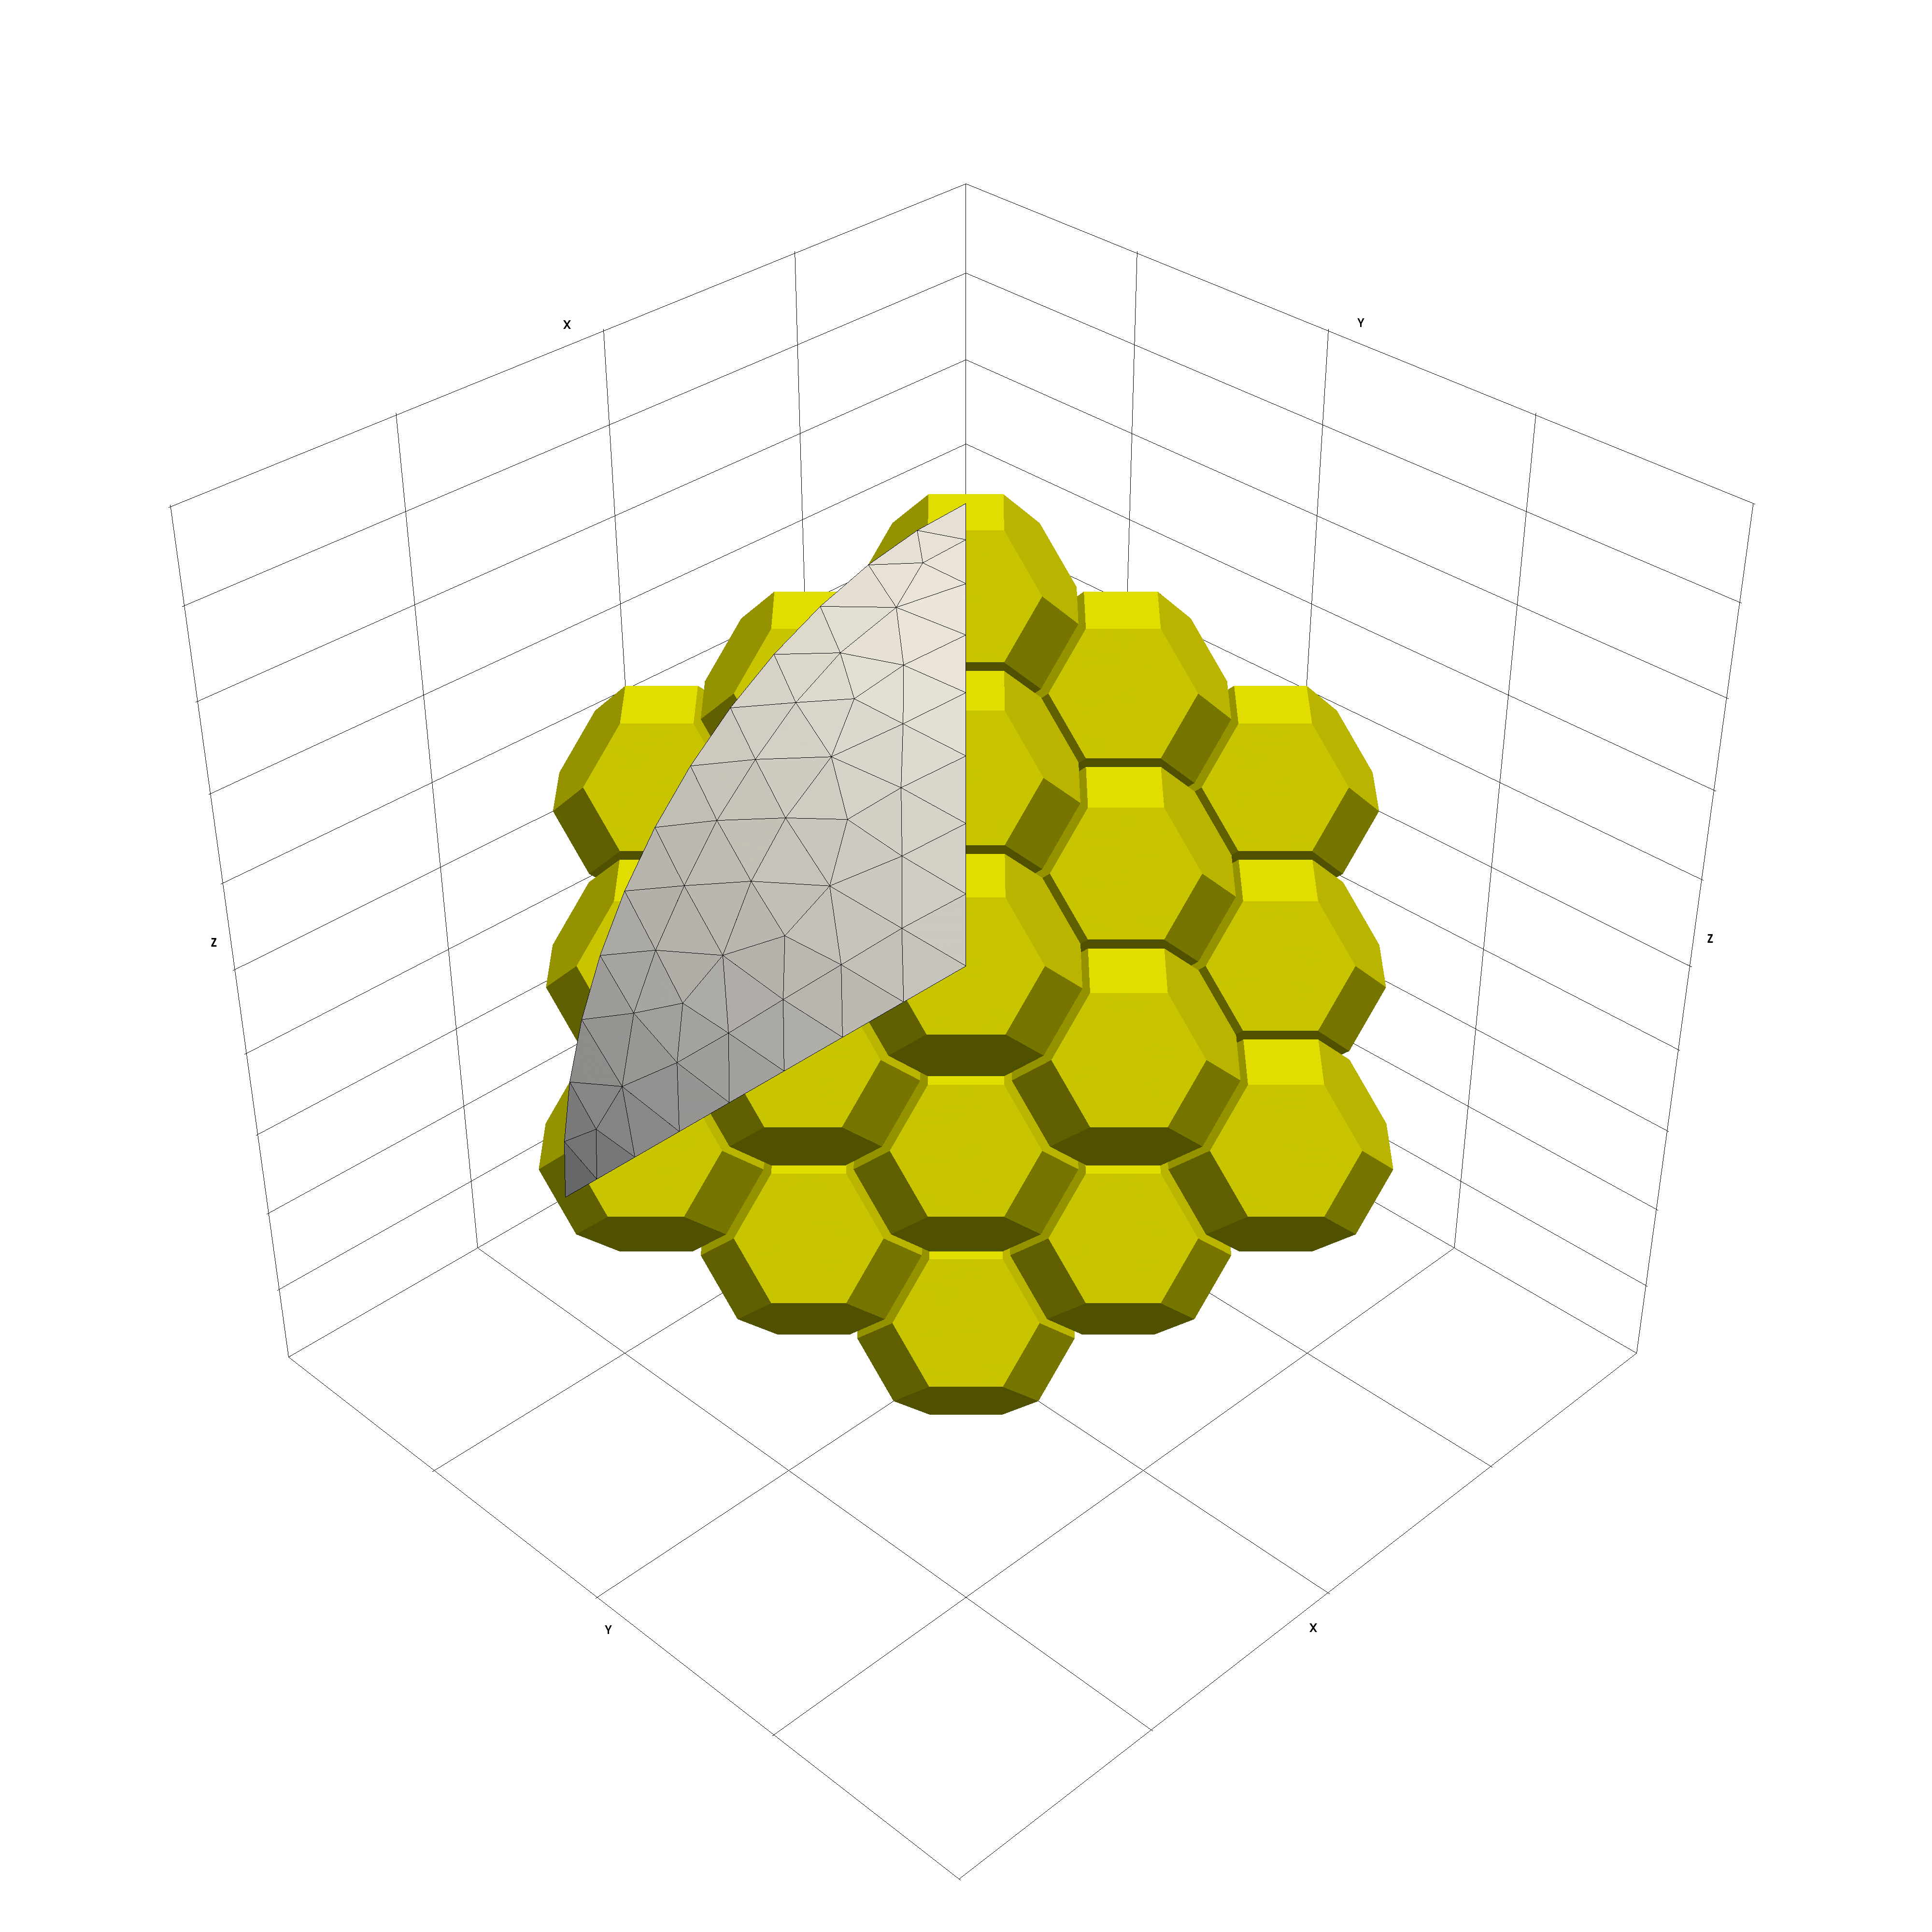
\includegraphics[width=\textwidth]{research-4/figs/mesh_orientations_HD.png}
\caption[Framboidal mesh and field orientations]{Framboidal mesh and field orientations.}
\label{FIG_01}
\end{figure}

\subsection{Mesh generation}
Outline of mesh generation. Explain the algorithm to produce arbitrarily large ordered framboidal meshes.\par

\section{Results}
Results section...\par

\subsection{The FORC diagrams}
Results of the hysteresis, FORCs and FORC diagrams. Explain here how the hysteresis curves (Figs. \ref{FIG_02}, \ref{FIG_04}, \ref{FIG_06}, \ref{FIG_08}) and FORC diagrams (Figs. \ref{FIG_03}, \ref{FIG_05}, \ref{FIG_07}, \ref{FIG_09}) depend on the field orientation. How the easy, hard axis are preserved in the framboidal structure (as compared to the isolated particles). Explain what the different FORC diagram features mean as switching fields of the individual particles in the framboids. Explain the FORCs (Fig. \ref{FIG_09}) and FORC diagram (Fig. \ref{FIG_10}) of the dispersion (ensemble average). Explain how FORC diagrams for mixtures of framboids and isolated SD particles (Fig. \ref{FIG_11}) and framboids and isolated SV particles (Fig. \ref{FIG_12}) were obtained (simple averages where the framboidal mass and isolated mass are the same). Explain how the framboids and the mixtures plot on the Day plot (Fig. \ref{FIG_14}).\par
\begin{figure}
\centering
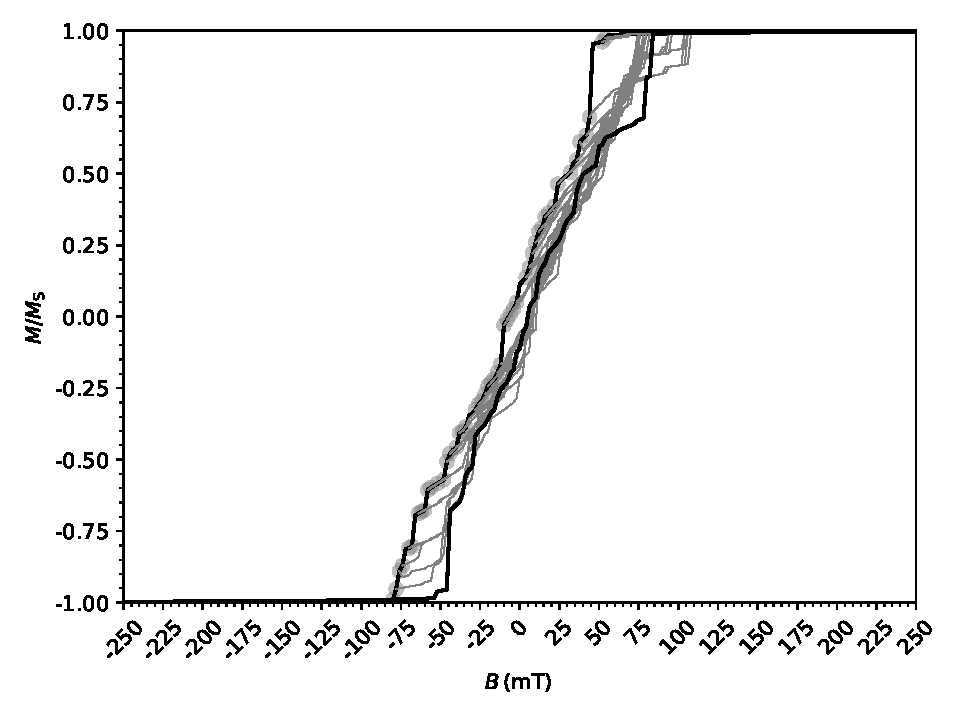
\includegraphics[width=\textwidth]{research-4/figs/BM21_withFORCS.pdf}
\caption[FORCs when the field is along an easy axis]{FORCs when the field is along an easy axis}.
\label{FIG_02}
\end{figure}

\begin{figure}
\centering
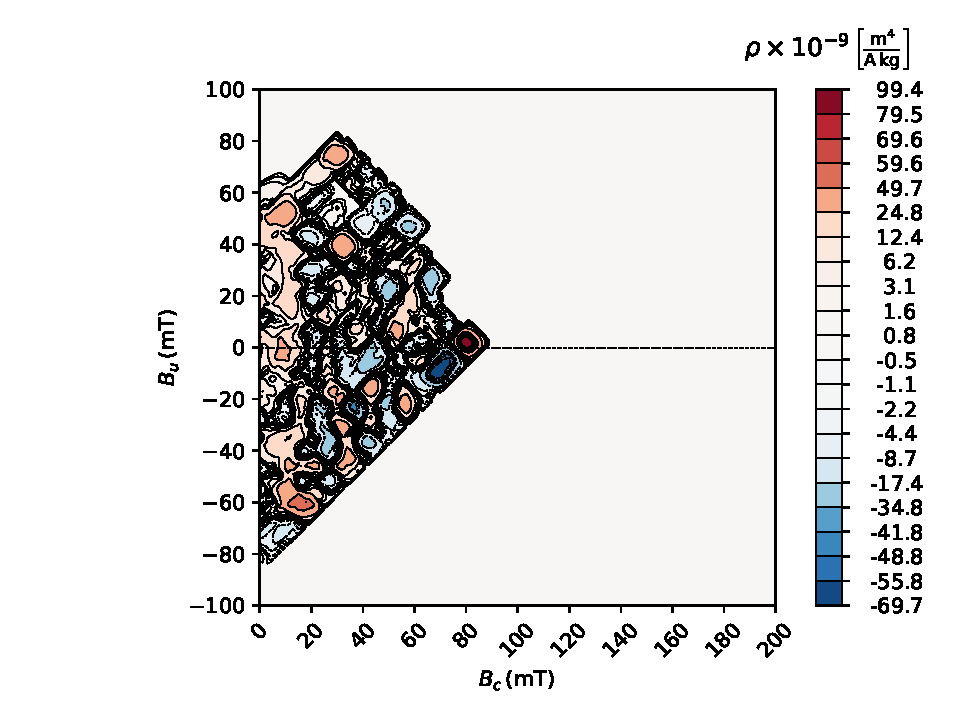
\includegraphics[width=\textwidth]{research-4/figs/FORC_21_SF4.pdf}
\caption[FORC diagram when the field is along an easy axis]{FORC diagram (SF=4) when the field is along an easy axis.}
\label{FIG_03}
\end{figure}

\begin{figure}
\centering
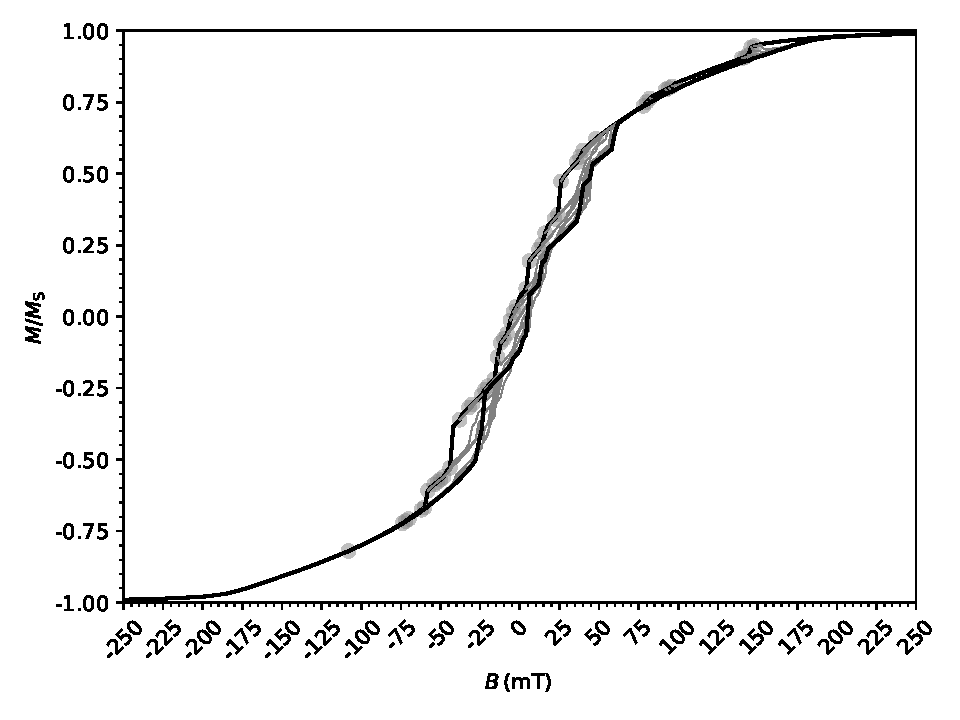
\includegraphics[width=\textwidth]{research-4/figs/BM16_withFORCS.pdf}
\caption[FORCs when the field is along a hard axis]{FORCs when the field is along a hard axis.}
\label{FIG_04}
\end{figure}

\begin{figure}
\centering
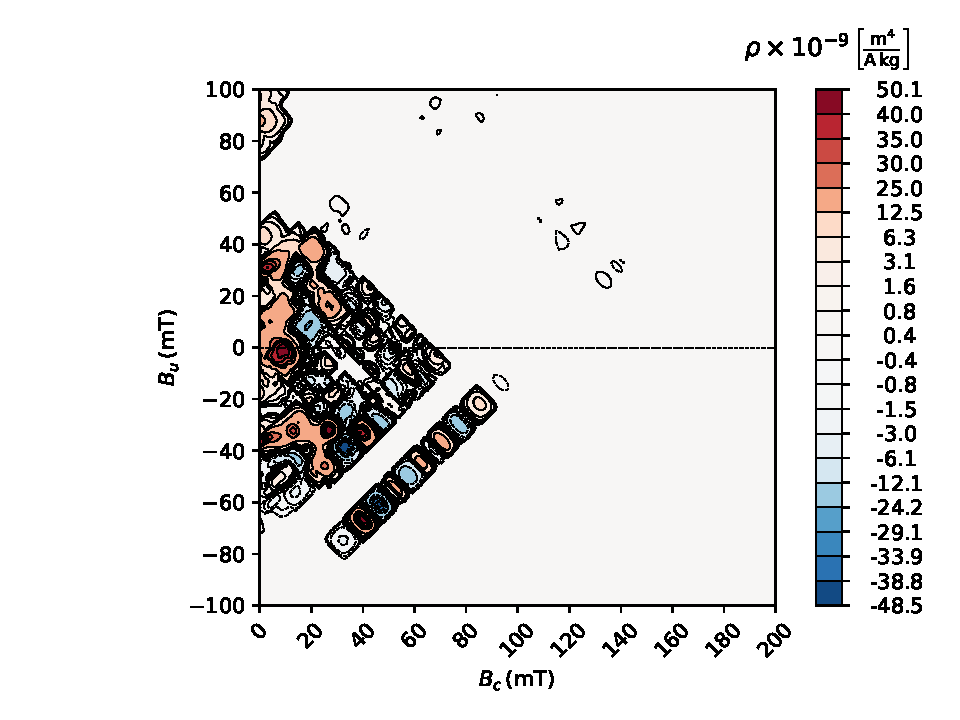
\includegraphics[width=\textwidth]{research-4/figs/FORC_16_SF4.pdf}
\caption[FORC diagram when the field is along a hard axis]{FORC diagram (SF=4) when the field is along a hard axis.}
\label{FIG_05}
\end{figure}

\begin{figure}
\centering
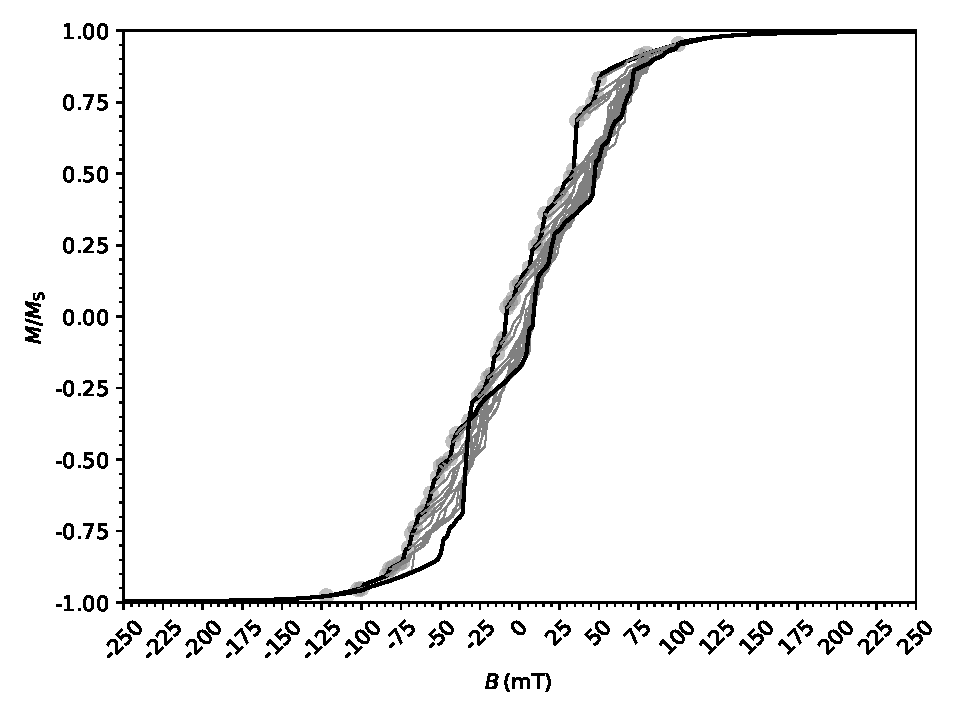
\includegraphics[width=\textwidth]{research-4/figs/BM14_withFORCS.pdf}
\caption[FORCs when the field is along a saddle point]{FORCs when the field is along a saddle point.}
\label{FIG_06}
\end{figure}

\begin{figure}
\centering
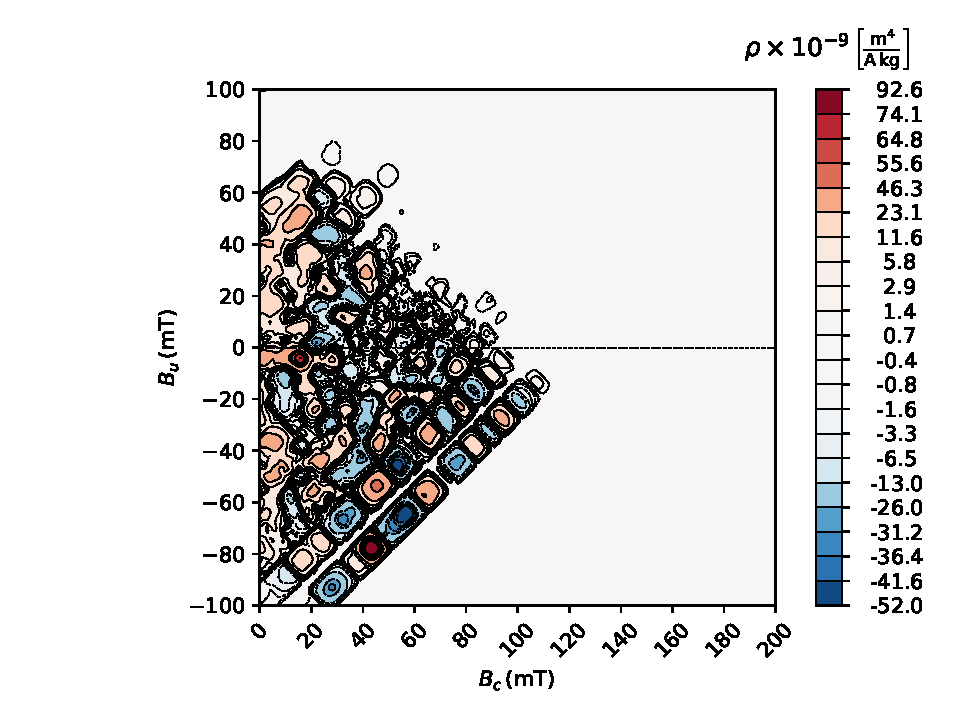
\includegraphics[width=\textwidth]{research-4/figs/FORC_14_SF4.pdf}
\caption[FORC diagram when the field is along a saddle point]{FORC diagram (SF=4) when the field is along a saddle point.}
\label{FIG_07}
\end{figure}

\begin{figure}
\centering
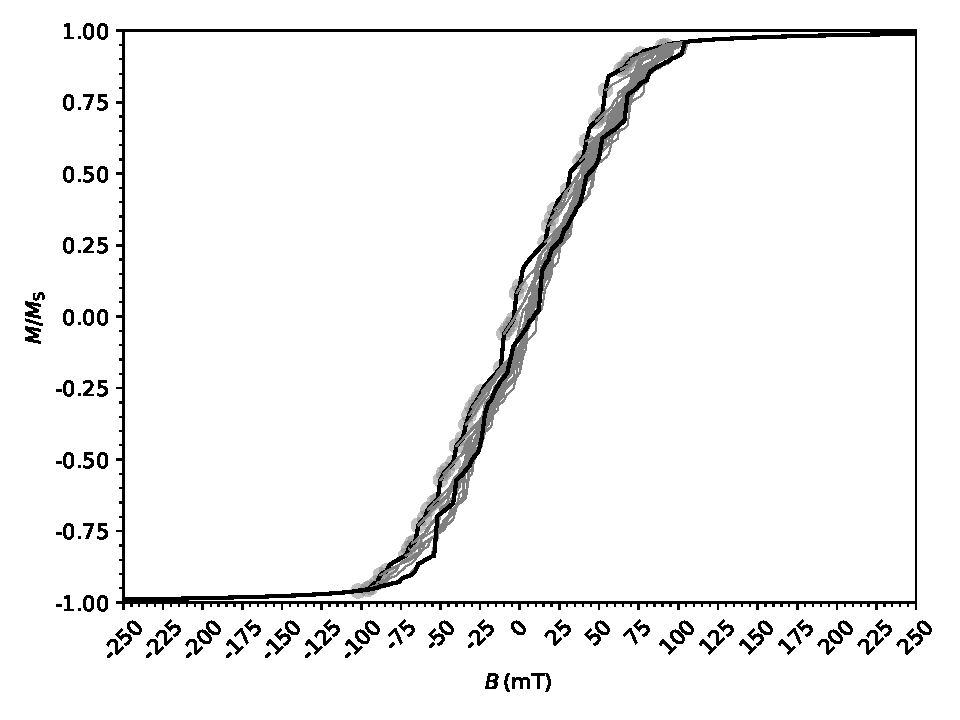
\includegraphics[width=\textwidth]{research-4/figs/BM53_withFORCS.pdf}
\caption[FORCs when the field is along a direction between easy, hard and saddle directions]{FORCs when the field is along a direction between easy, hard and saddle directions.}
\label{FIG_08}
\end{figure}

\begin{figure}
\centering
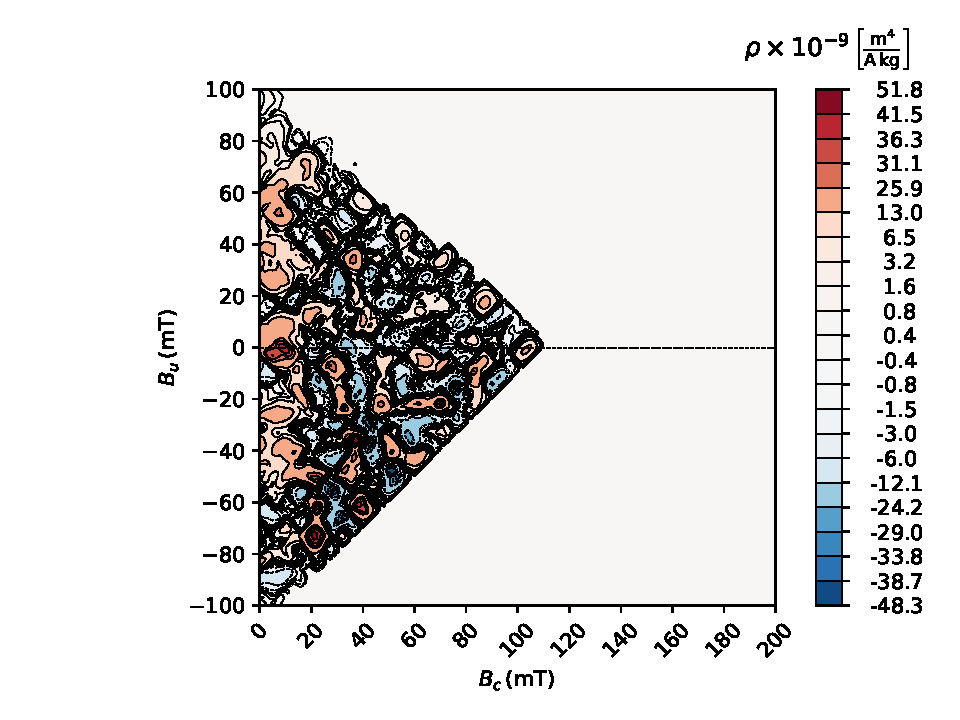
\includegraphics[width=\textwidth]{research-4/figs/FORC_53_SF4.pdf}
\caption[FORC diagram when the field is along a direction between easy, hard and saddle directions]{FORC diagram (SF=4) when the field is along a direction between easy, hard and saddle directions.}
\label{FIG_09}
\end{figure}

\begin{figure}
\centering
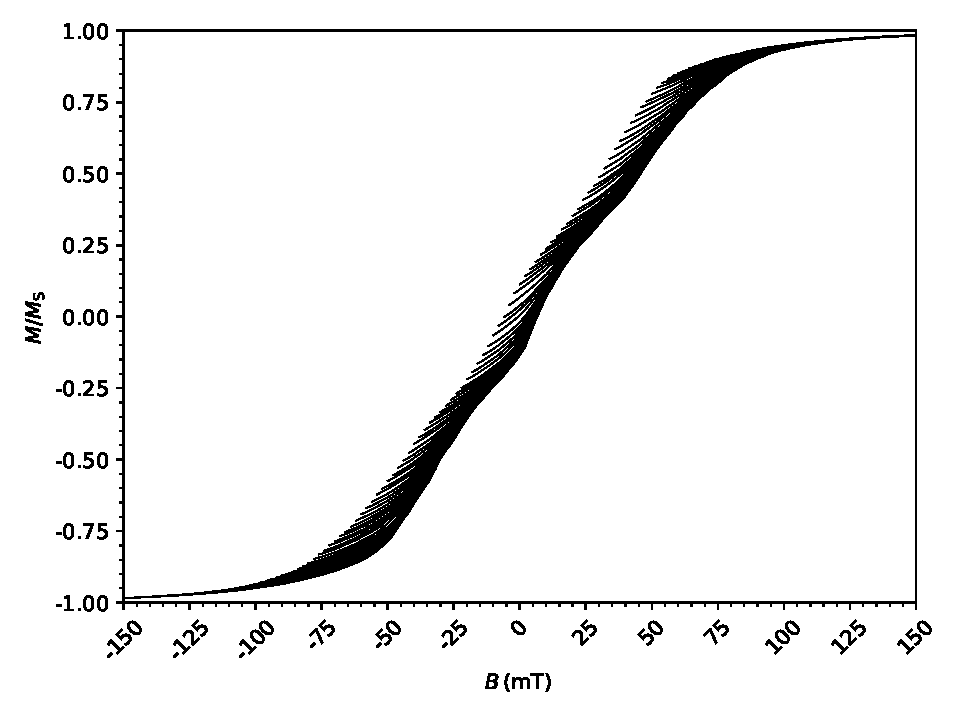
\includegraphics[width=\textwidth]{research-4/figs/BM_fram_avg.pdf}
\caption[FORCs of the framboid dispersion]{FORCs of the framboid dispersion.}
\label{FIG_10}
\end{figure}

\begin{figure}
\centering
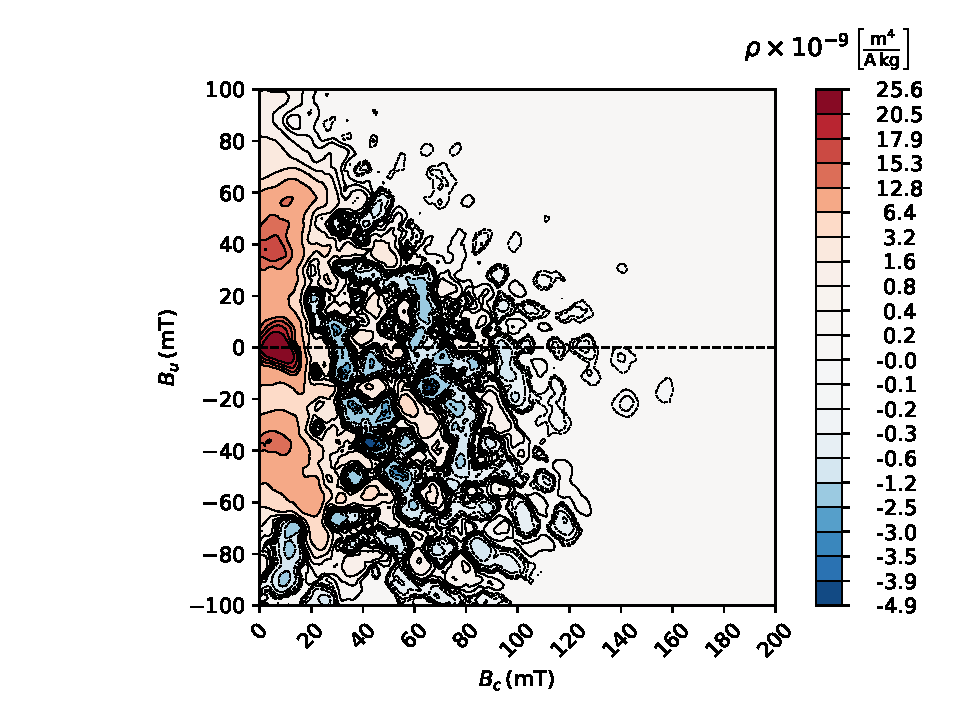
\includegraphics[width=\textwidth]{research-4/figs/FORC_framAVG_SF4.pdf}
\caption[FORC diagram of the framboid dispersion]{FORC diagram (SF=4) of the framboid dispersion.}
\label{FIG_11}
\end{figure}

\begin{figure}
\centering
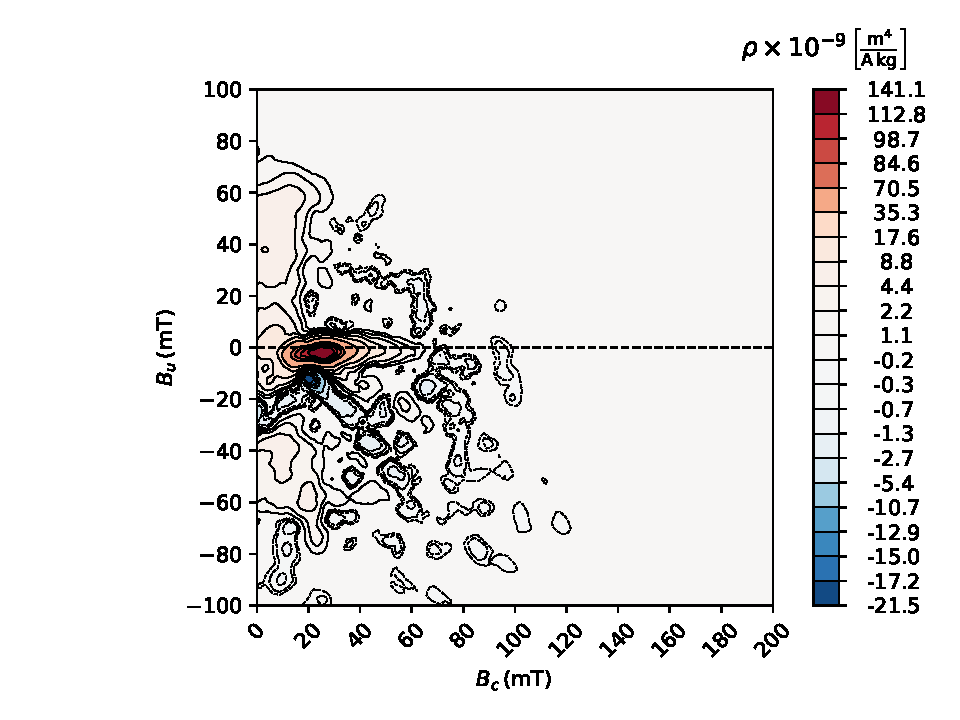
\includegraphics[width=\textwidth]{research-4/figs/FORC_framAVG_SF4_mixed_SD_ratio1.pdf}
\caption[FORCs of a dispersion of framboids and noninteracting SD particles]{FORCs of a dispersion of framboids and noninteracting particles.}
\label{FIG_12}
\end{figure}

\begin{figure}
\centering
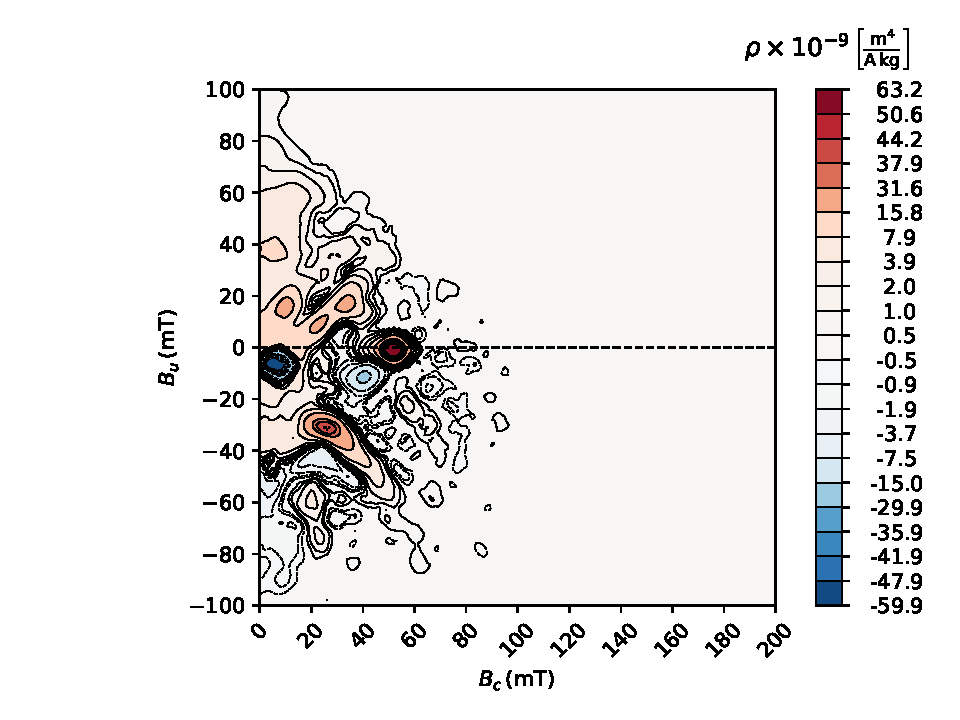
\includegraphics[width=\textwidth]{research-4/figs/FORC_framAVG_SF4_mixed_vortex_ratio1.pdf}
\caption[FORCs of a dispersion of framboids and noninteracting SV particles]{FORCs of a dispersion of framboids and noninteracting SV particles.}
\label{FIG_13}
\end{figure}

\begin{figure}
\centering
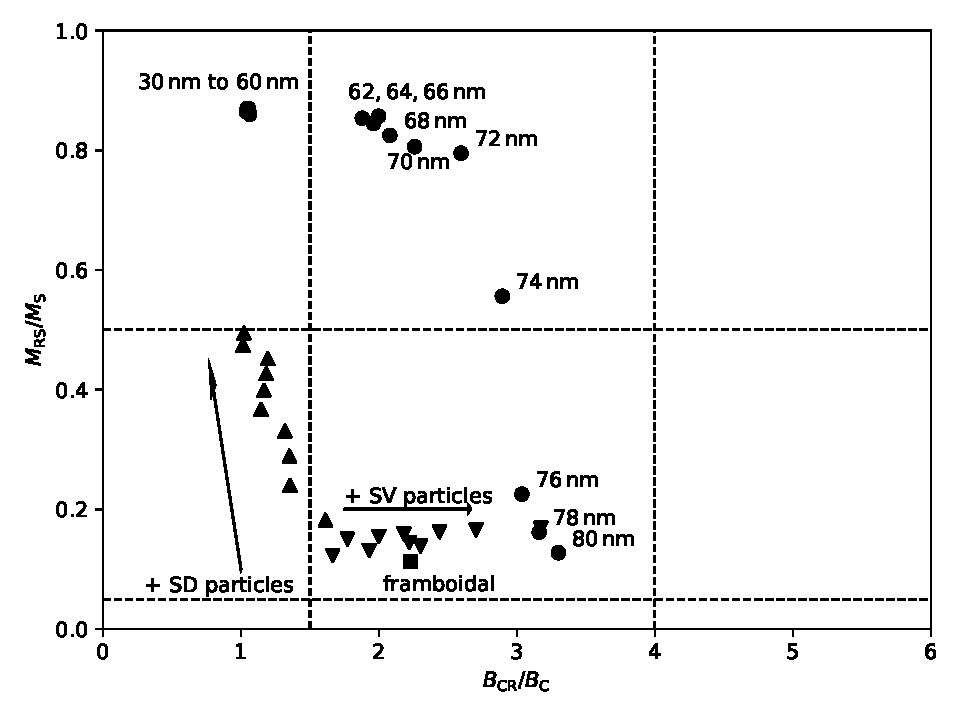
\includegraphics[width=\textwidth]{research-4/figs/DayPlot.pdf}
\caption[Day plot of framboid and noninteraring particles mixtures]{Day plot of framboid and noninteraring particles mixtures.}
\label{FIG_14}
\end{figure}

\subsection{Remanent states}
The remanent states, micromagnetic solutions and electron holography maps. Explain about the remanent states and how they would appear under electron holography studies. Important to stress how the electron holography maps can be misleading as evidenced by Figs. \ref{FIG_21}, \ref{FIG_22}, \ref{FIG_23}, \ref{FIG_24}, \ref{FIG_25}, \ref{FIG_26} which show either a single-vortex or a two-vortex structure depending on the angle of the beam.\par
\begin{figure}
\centering
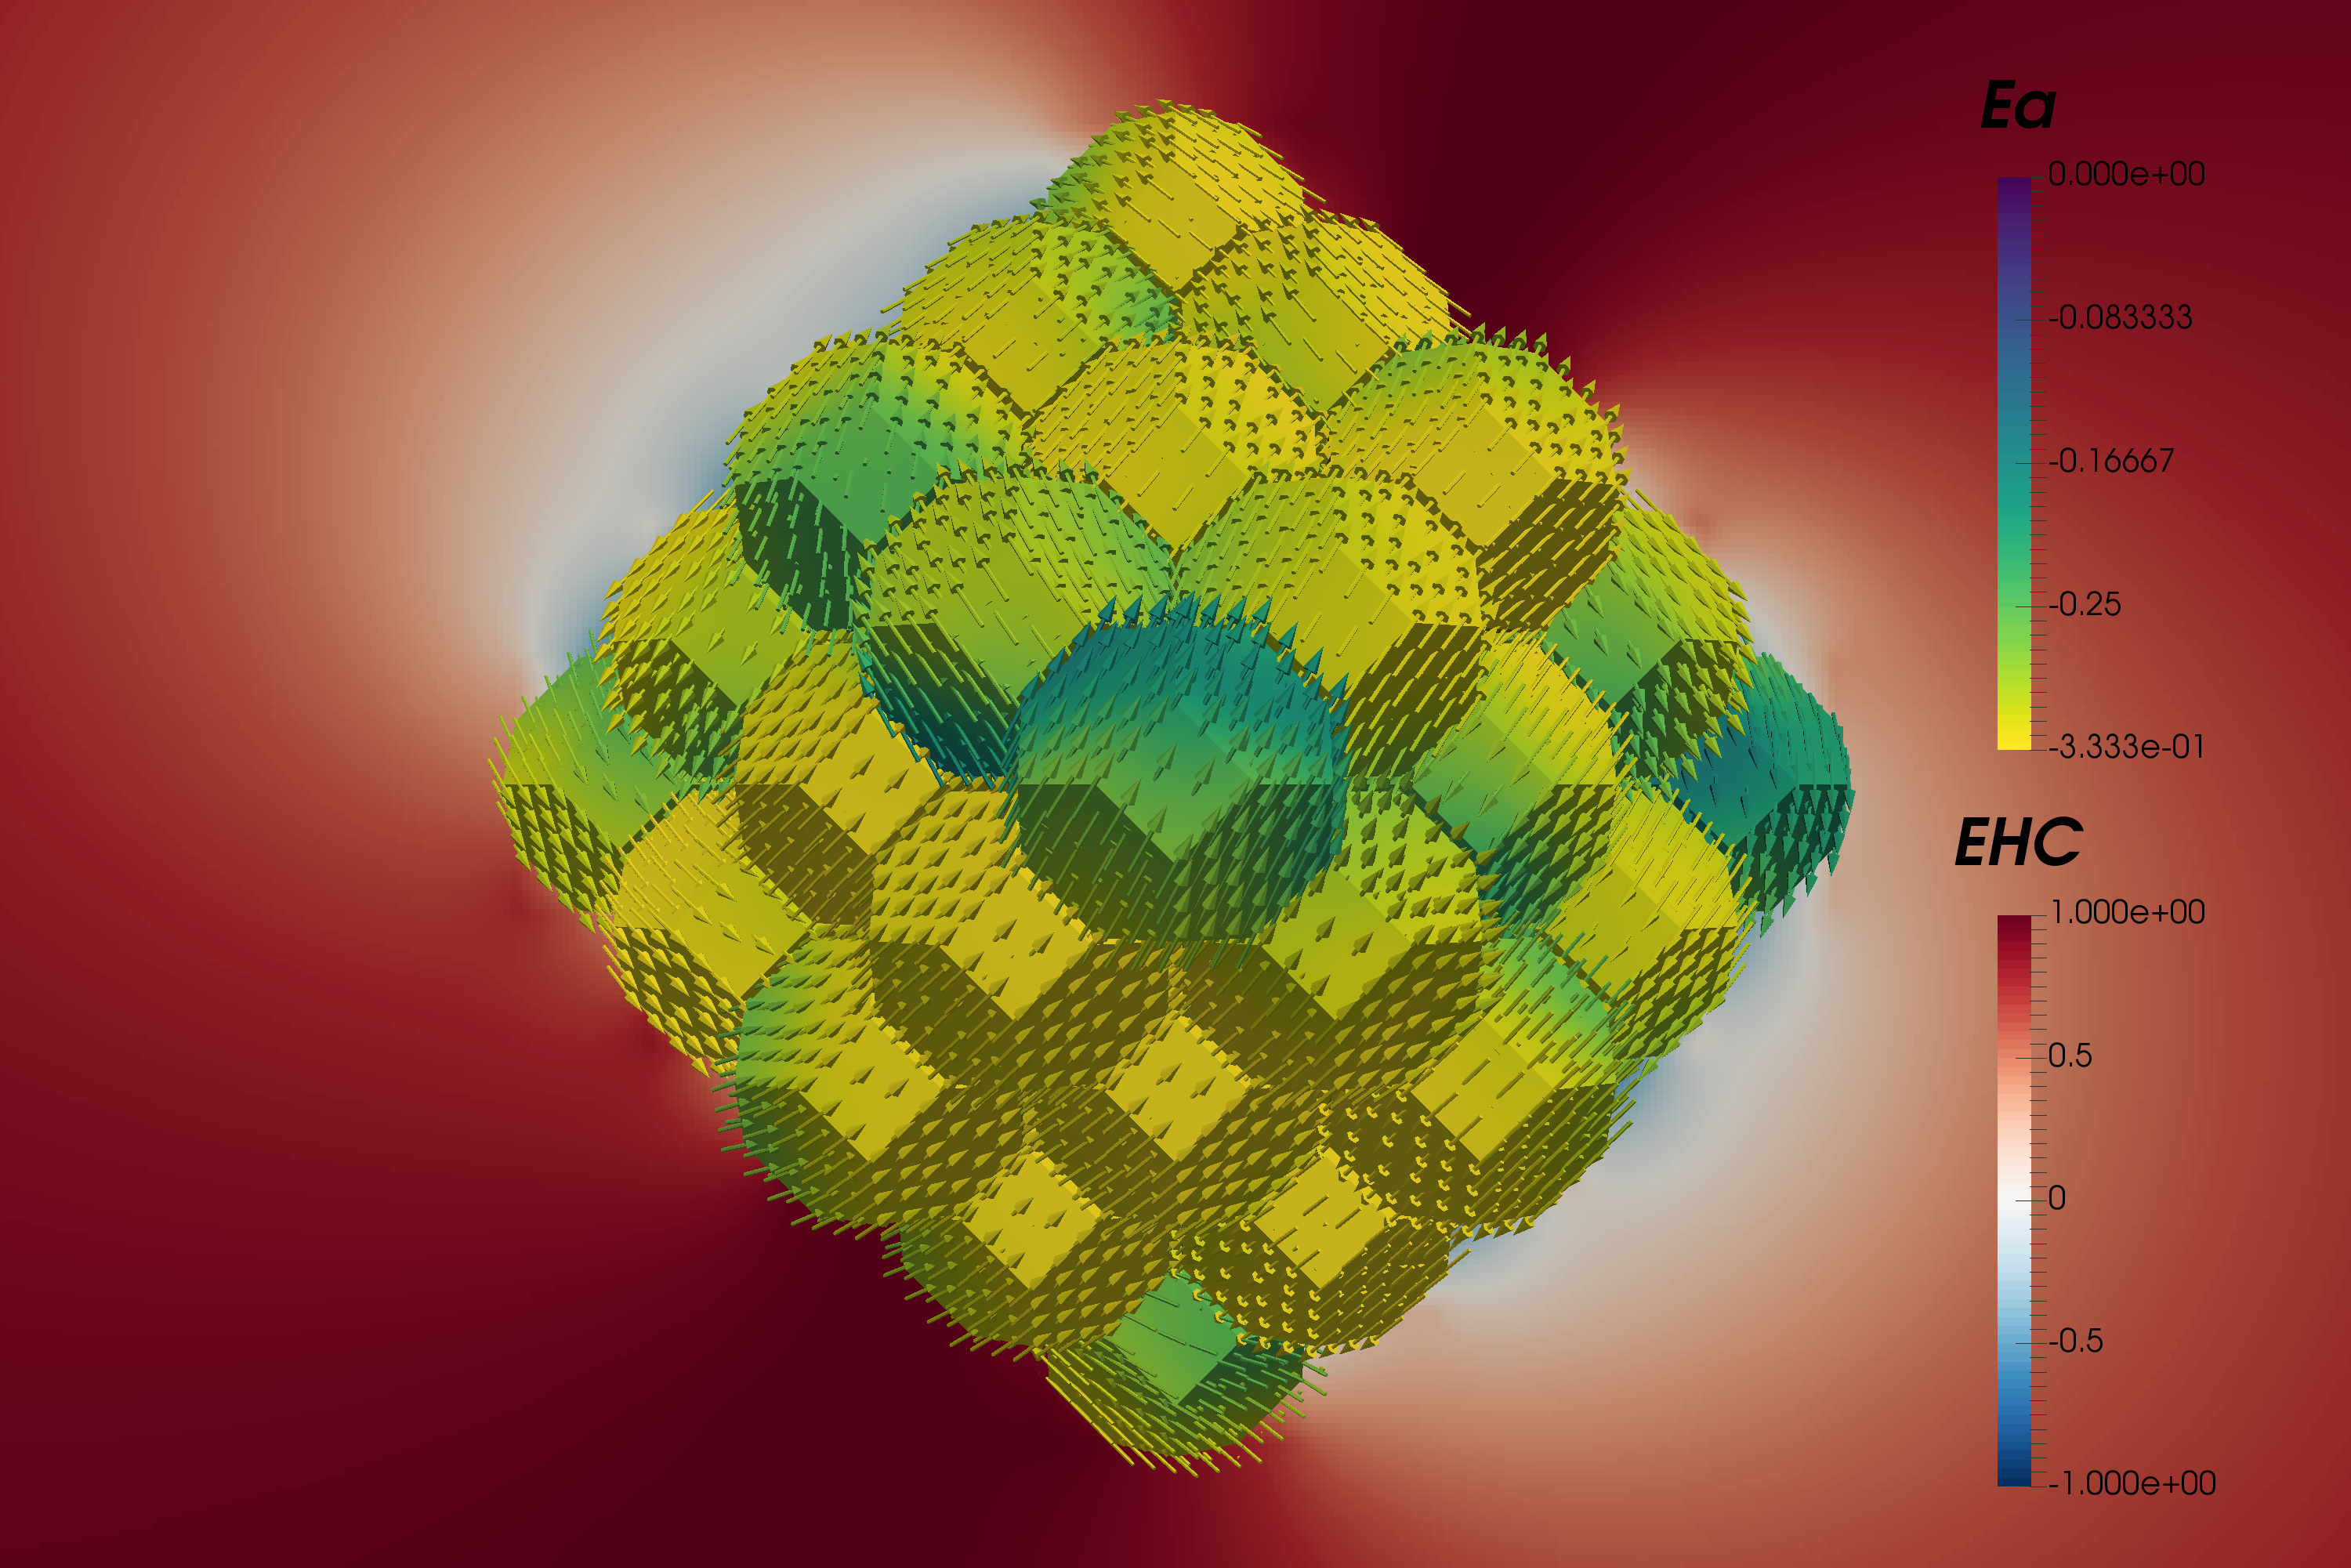
\includegraphics[width=\textwidth]{research-4/figs/fram_i21_f0_-z.png}
\caption[Remanent state when the field is along an easy axis (view from +Z)]{Remanent state when the field is along an easy axis (view from +Z).}
\label{FIG_15}
\end{figure}

\begin{figure}
\centering
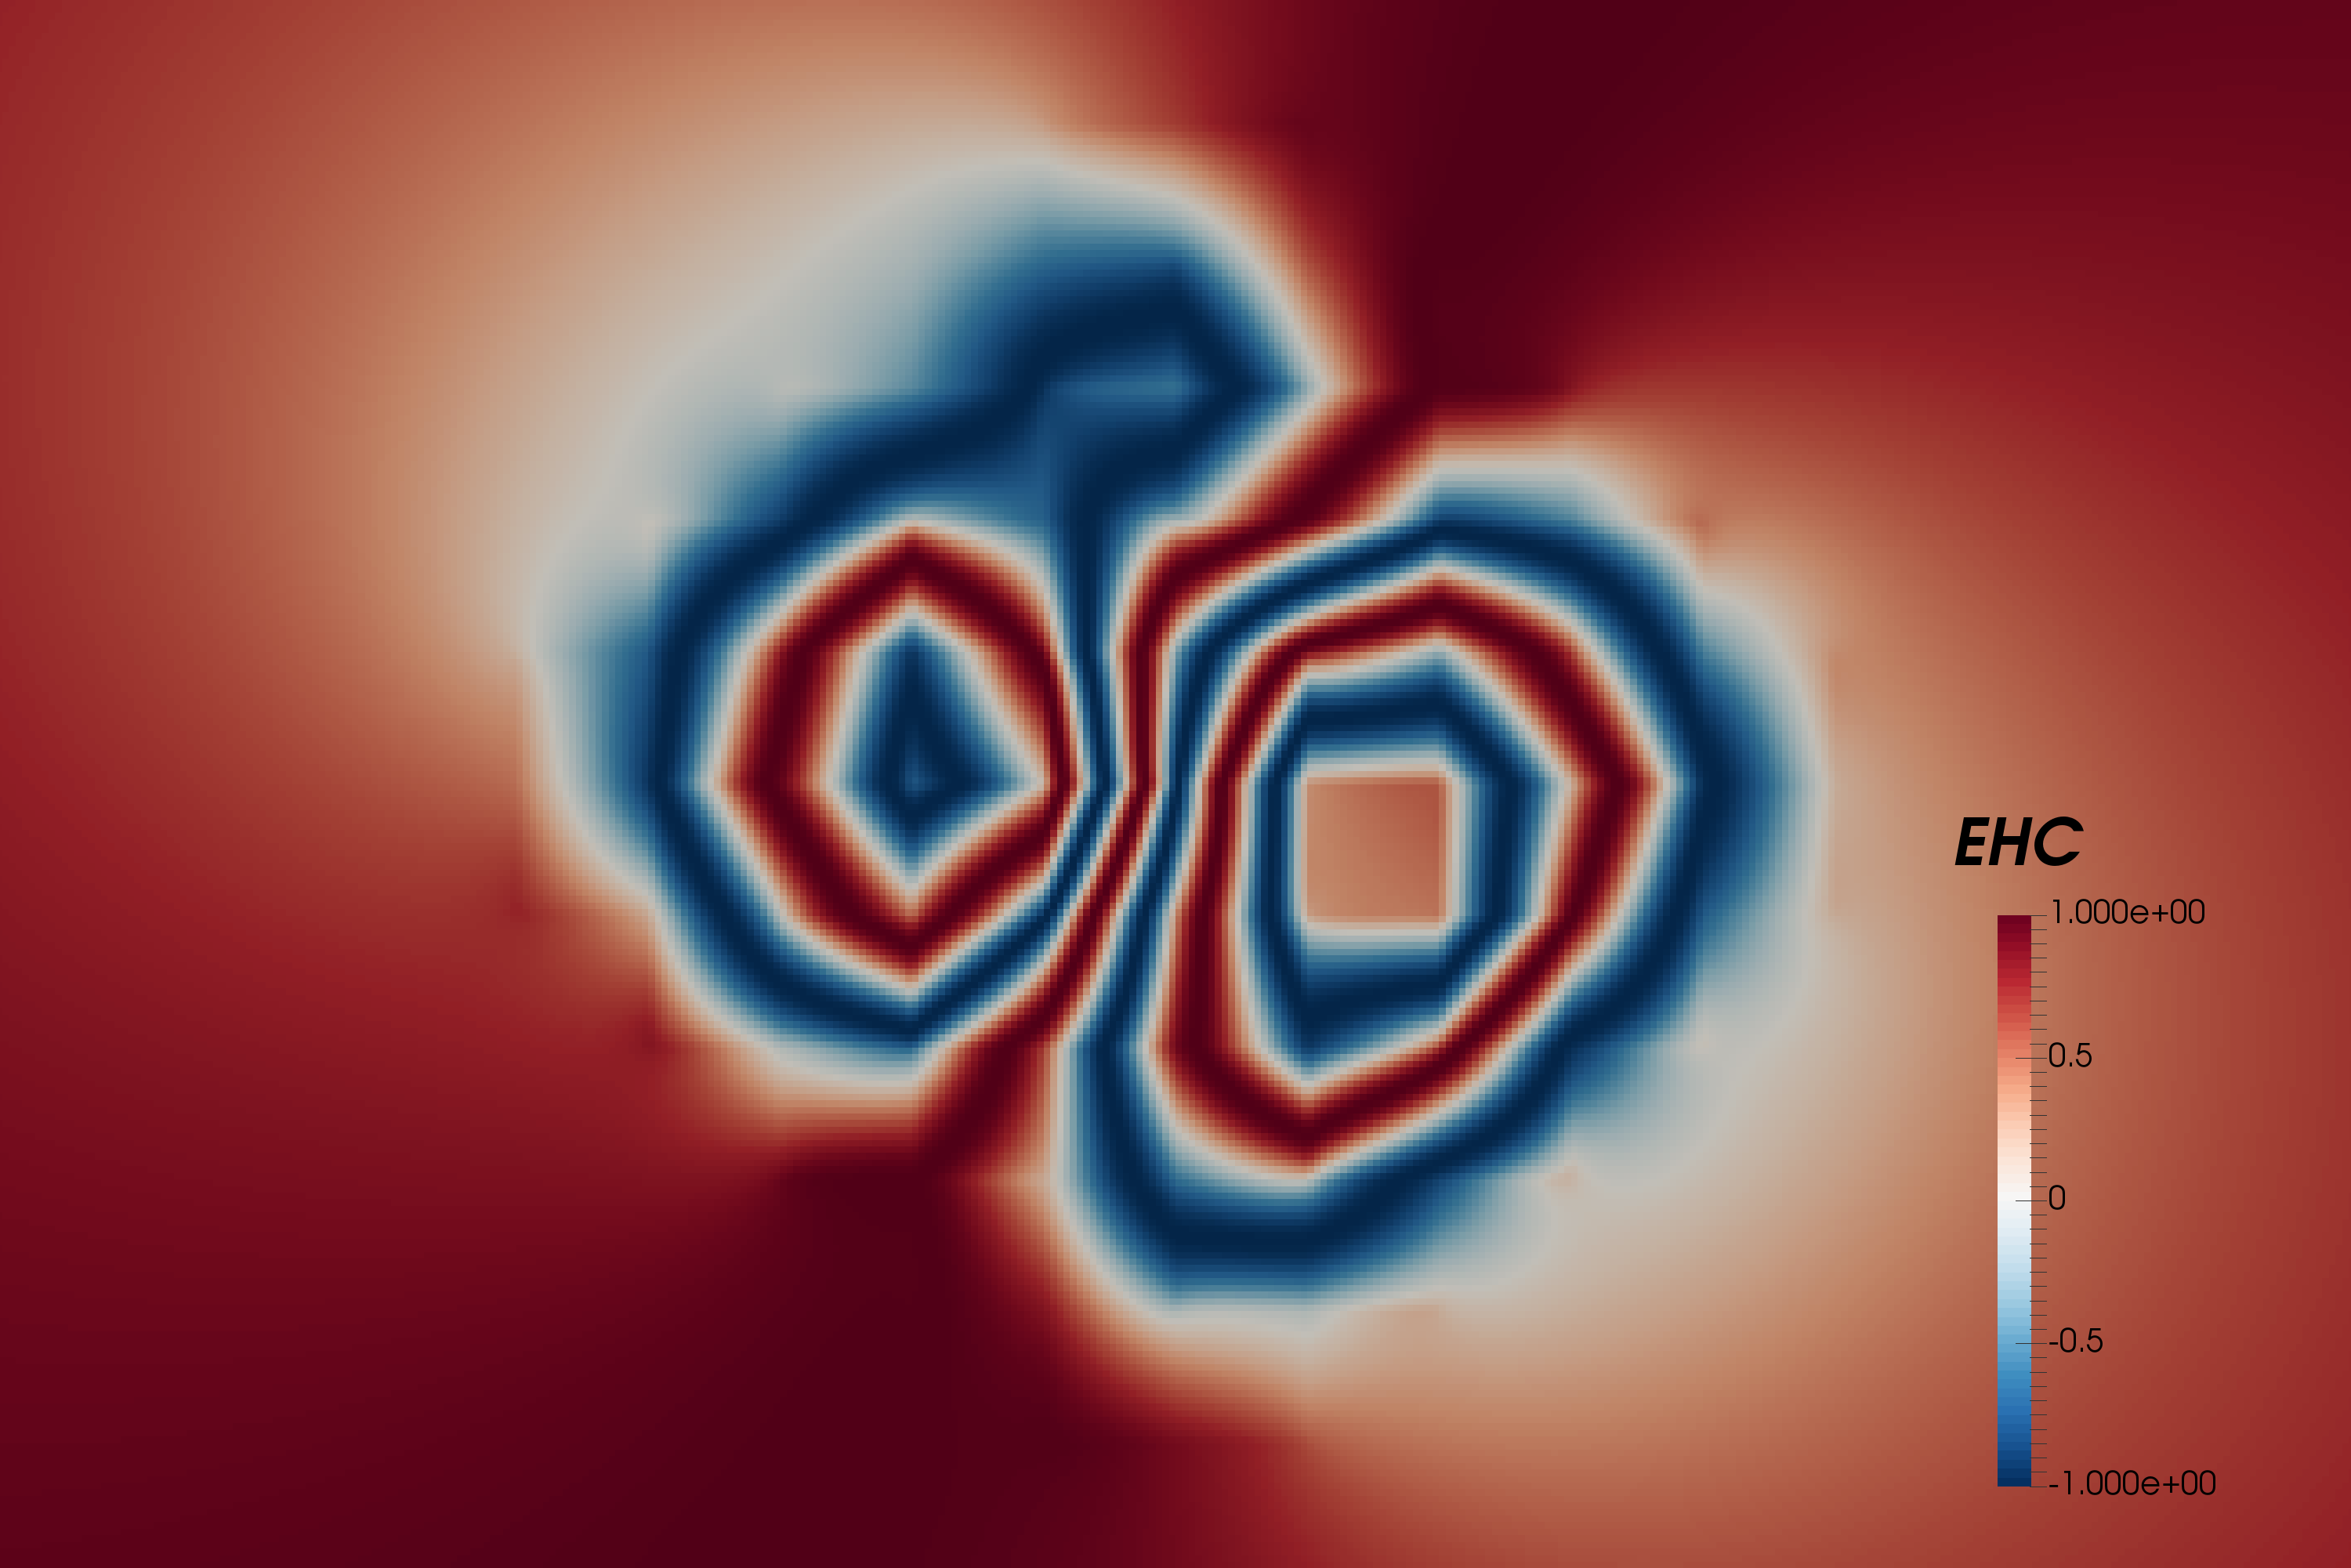
\includegraphics[width=\textwidth]{research-4/figs/fram_i21_f0_-z_EHC.png}
\caption[Electron holography map of the remanent state when the field is along an easy axis (view from +Z)]{Electron holography map of the remanent state when the field is along an easy axis (view from +Z).}
\label{FIG_16}
\end{figure}

\begin{figure}
\centering
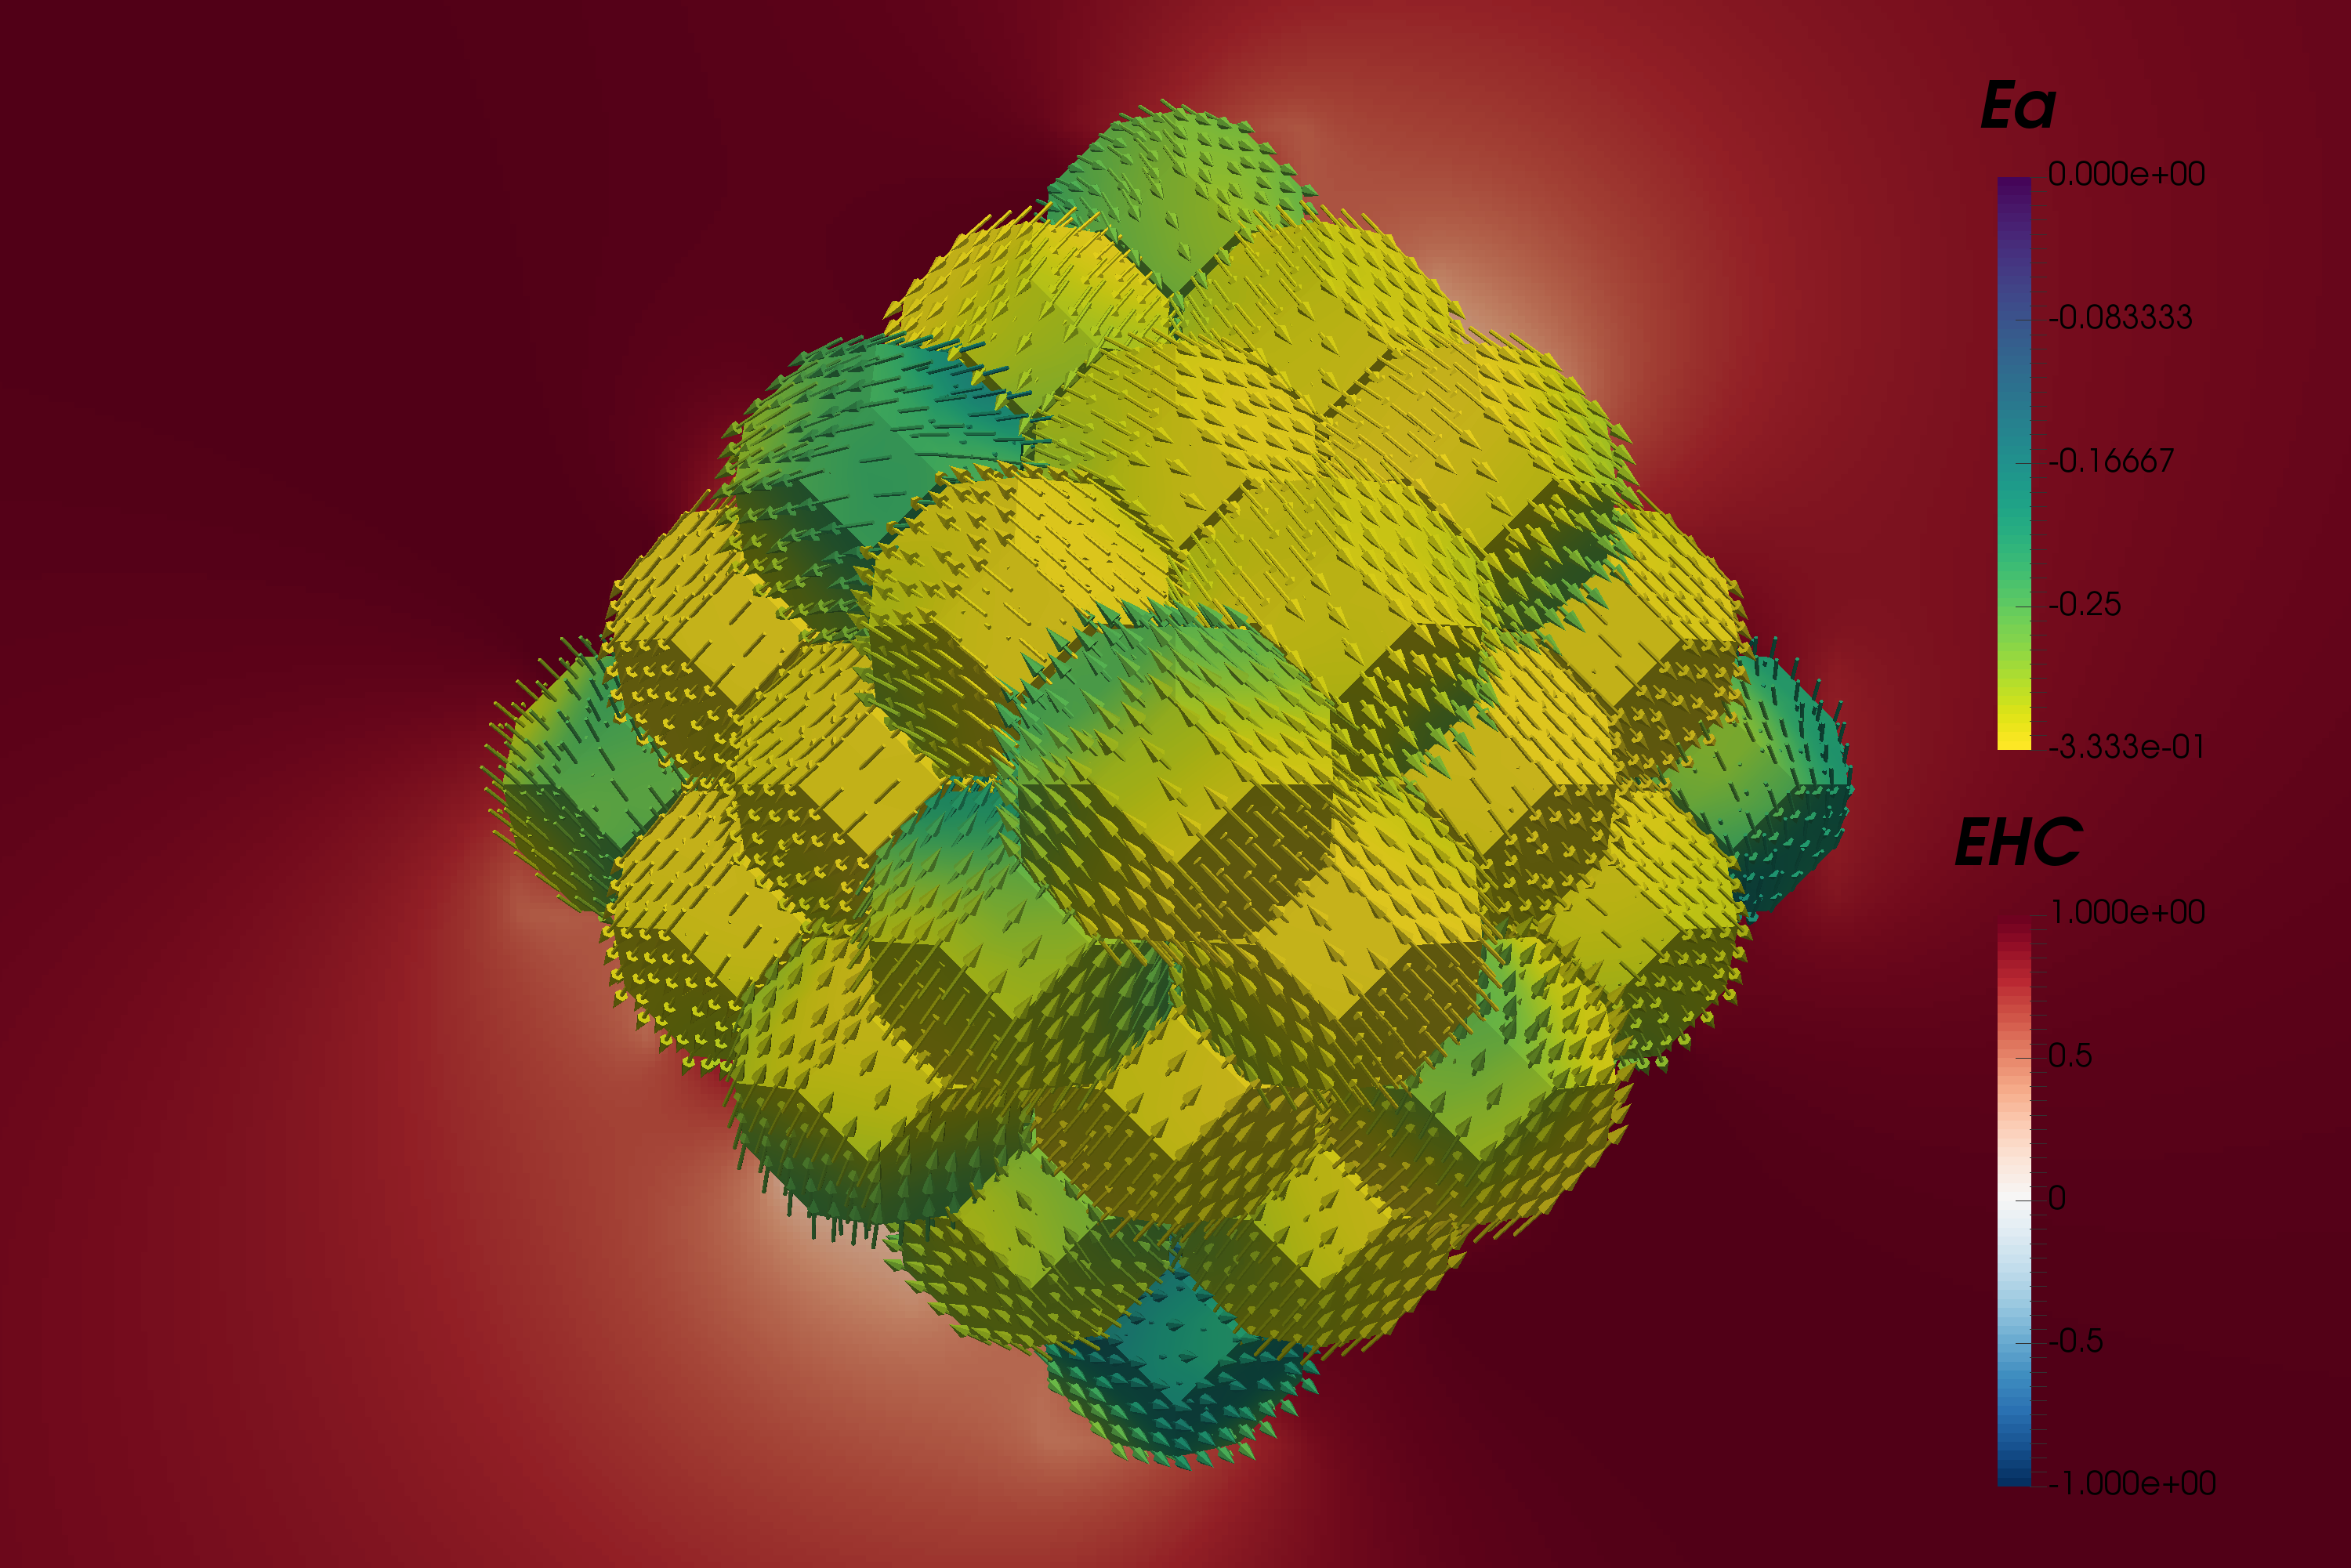
\includegraphics[width=\textwidth]{research-4/figs/fram_i21_f0_-y.png}
\caption[Remanent state when the field is along an easy axis (view from +Y)]{Remanent state when the field is along an easy axis (view from +Y).}
\label{FIG_17}
\end{figure}

\begin{figure}
\centering
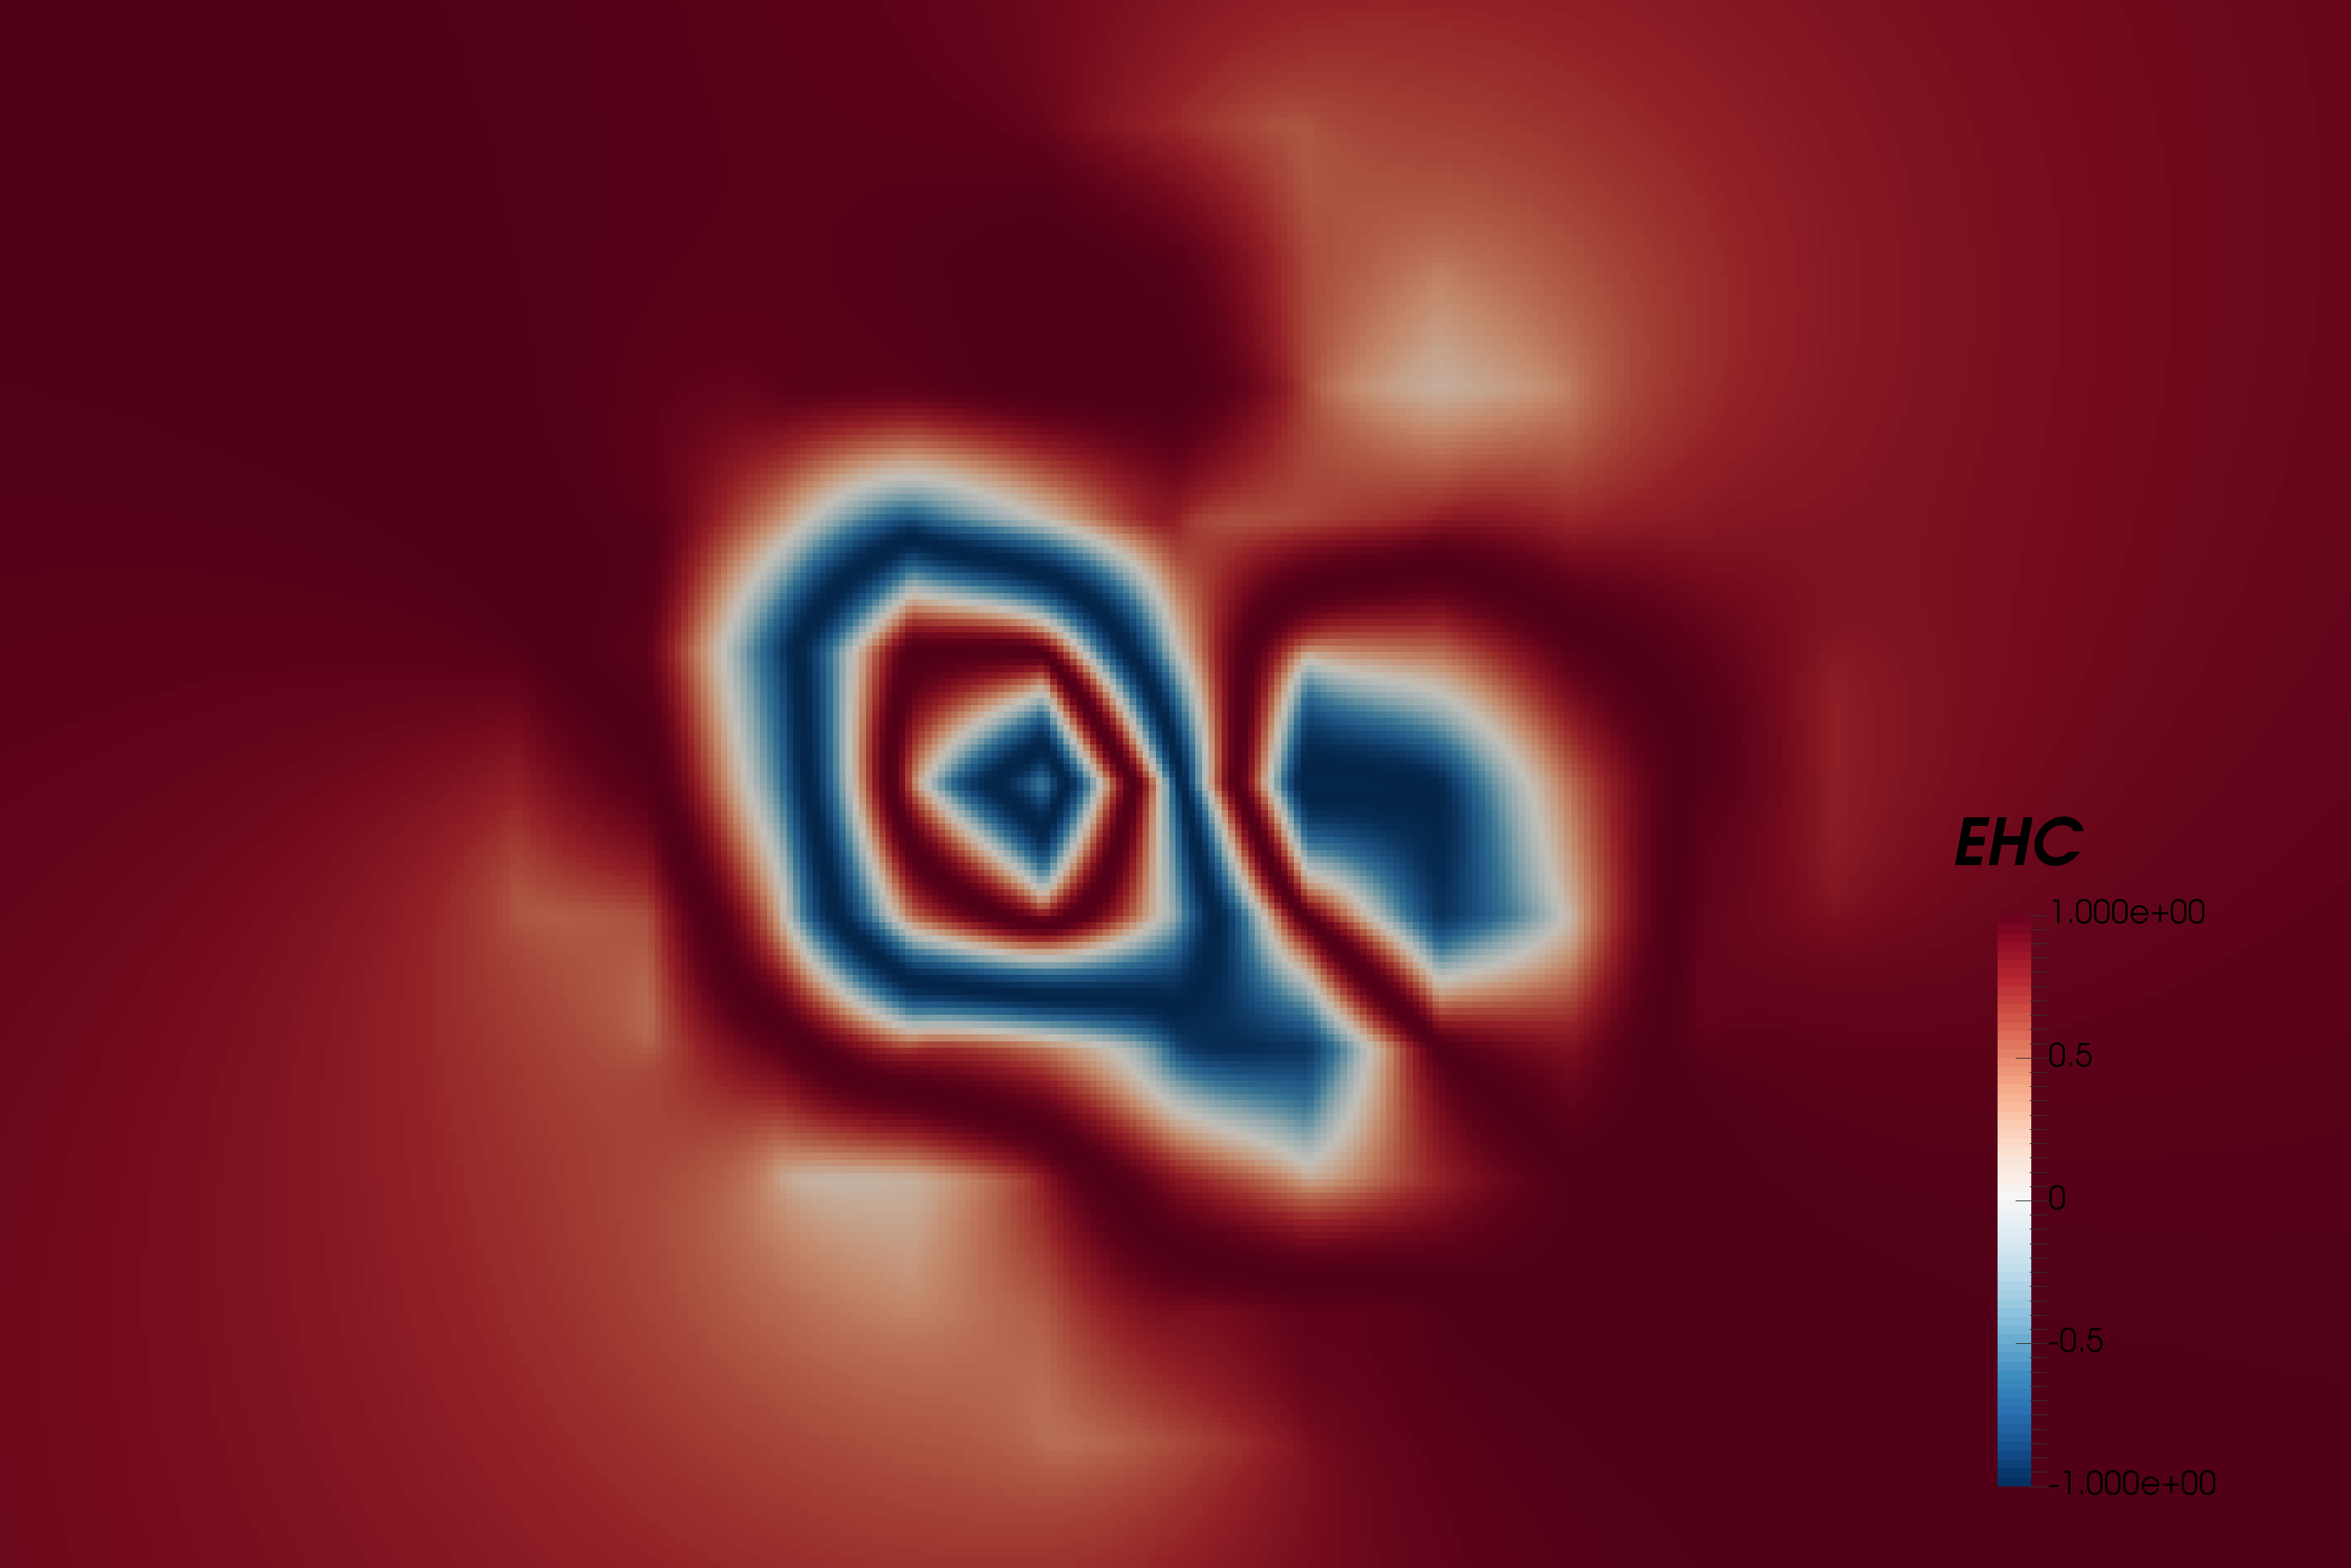
\includegraphics[width=\textwidth]{research-4/figs/fram_i21_f0_-y_EHC.png}
\caption[Electron holography map of the remanent state when the field is along an easy axis (view from +Y)]{Electron holography map of the remanent state when the field is along an easy axis (view from +Y).}
\label{FIG_18}
\end{figure}

\begin{figure}
\centering
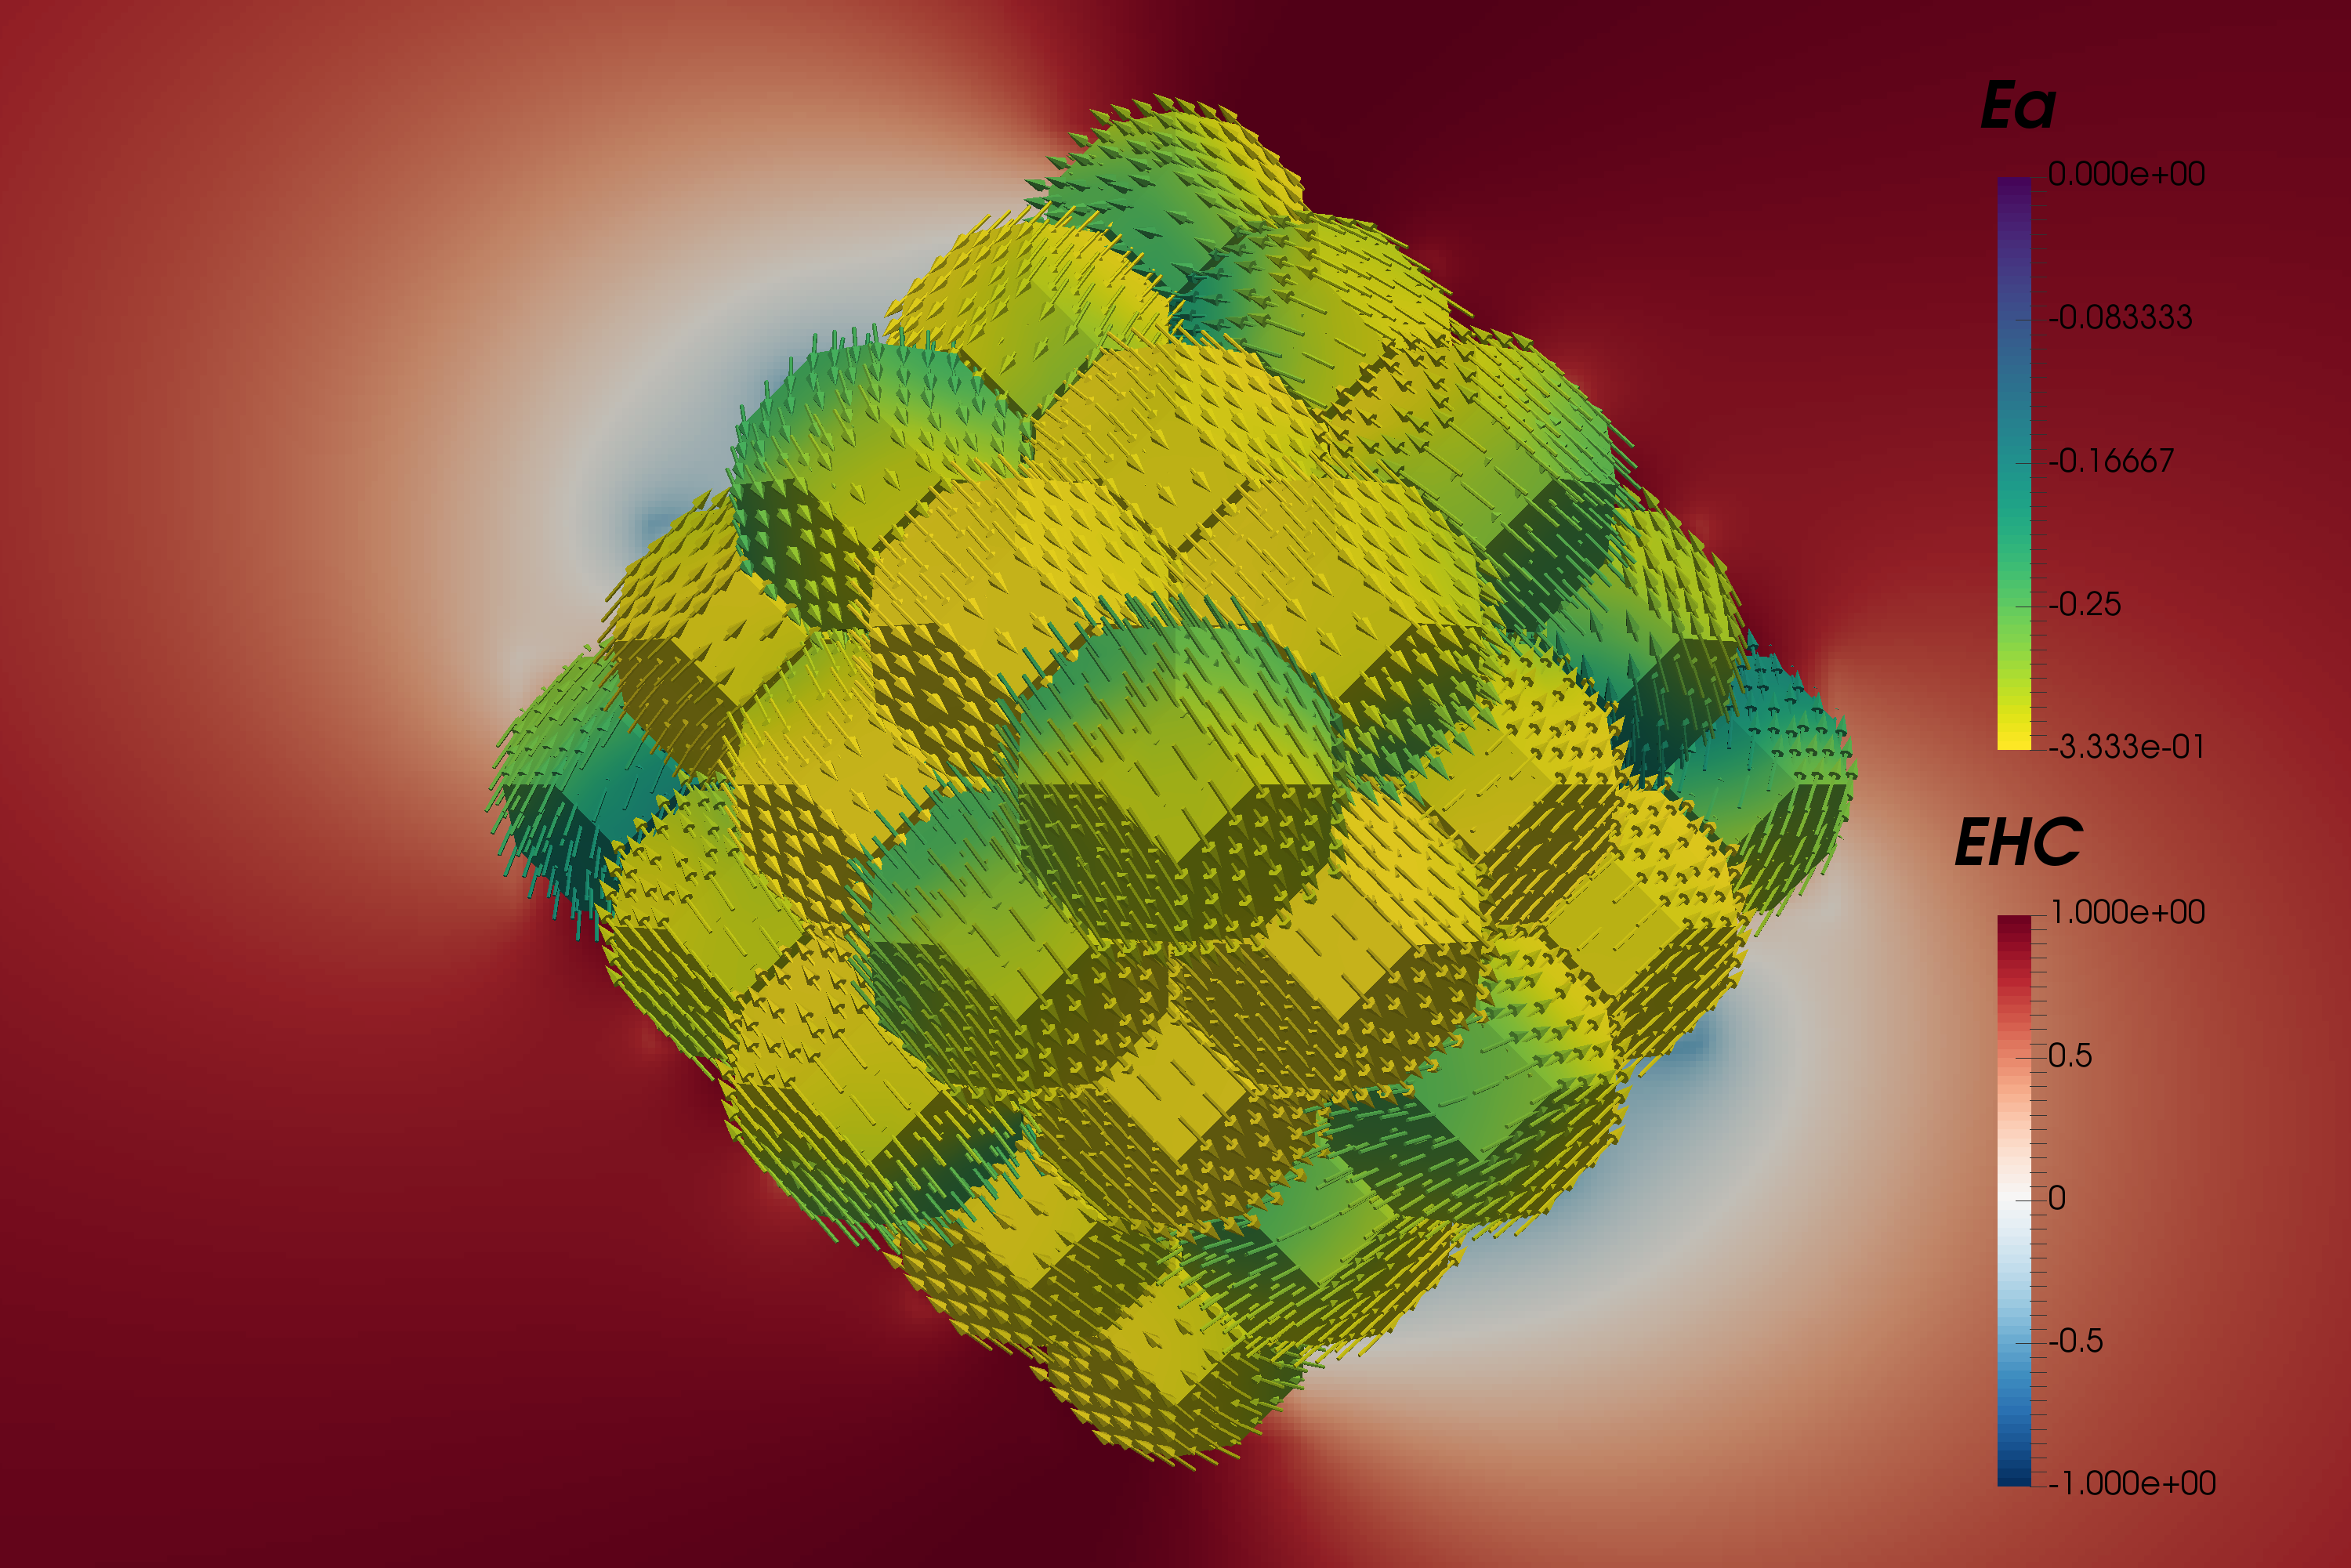
\includegraphics[width=\textwidth]{research-4/figs/fram_i21_f0_-x.png}
\caption[Remanent state when the field is along an easy axis (view from +X)]{Remanent state when the field is along an easy axis (view from +X).}
\label{FIG_19}
\end{figure}

\begin{figure}
\centering
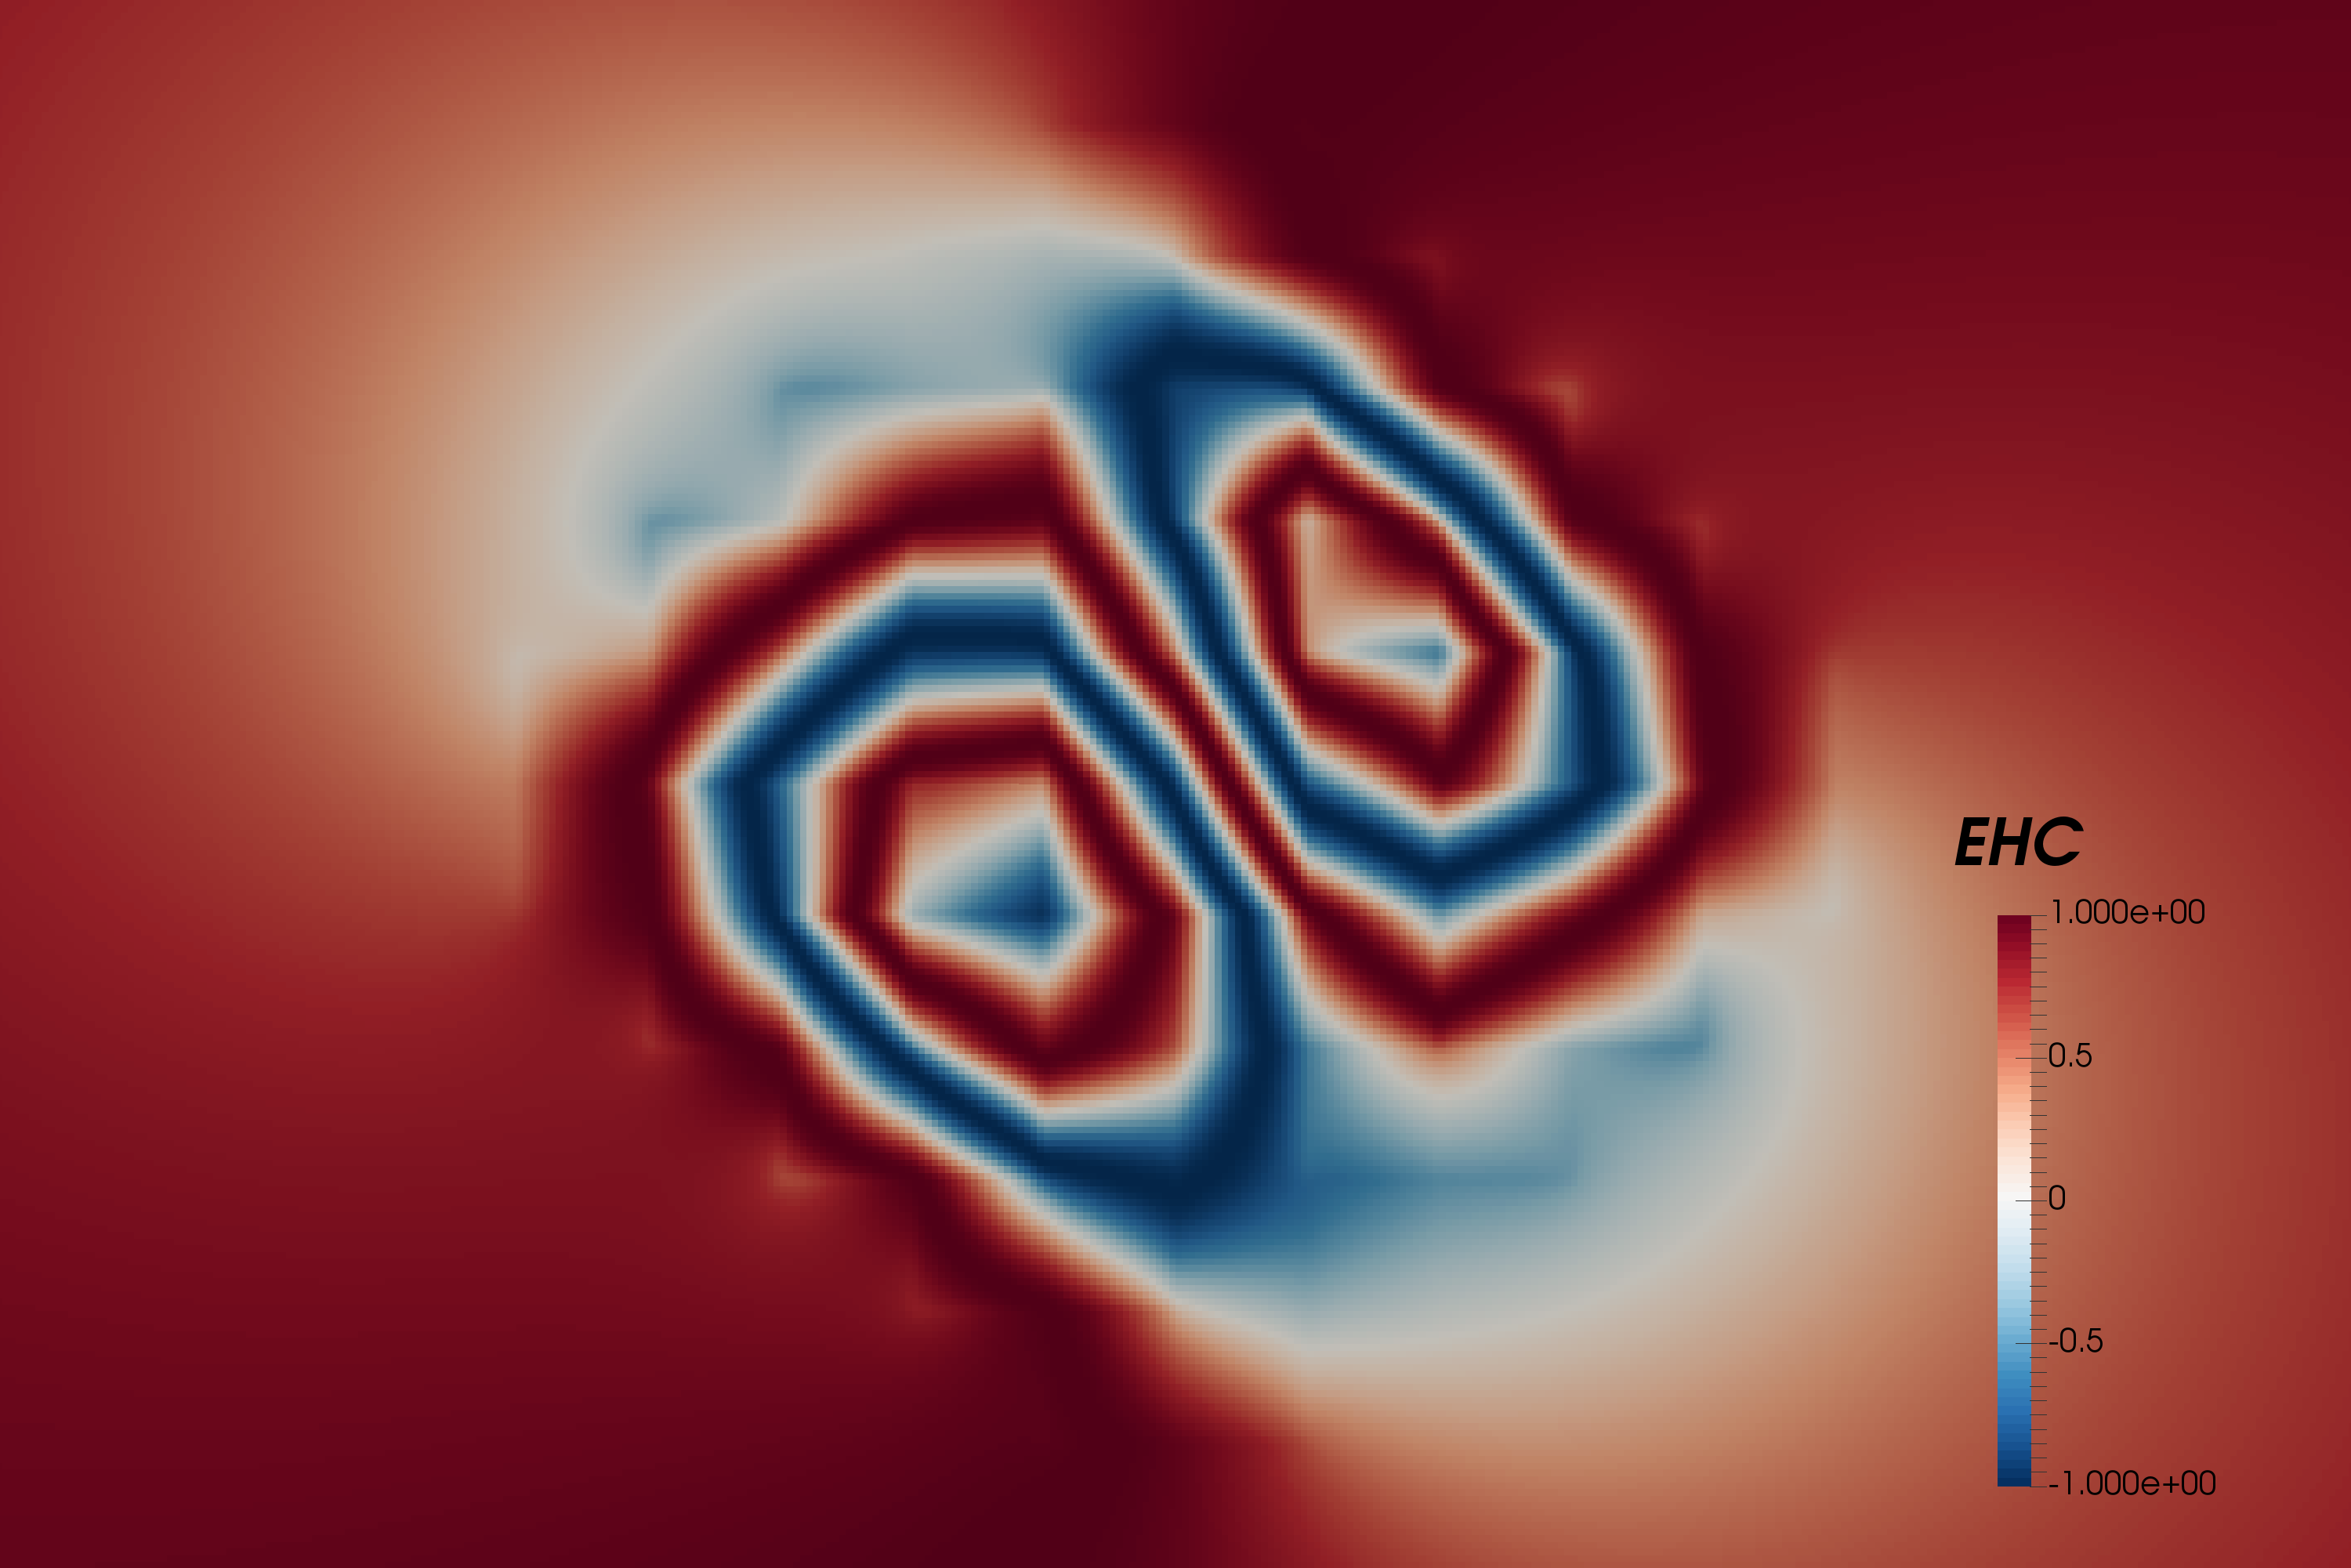
\includegraphics[width=\textwidth]{research-4/figs/fram_i21_f0_-x_EHC.png}
\caption[Electron holography map of the remanent state when the field is along an easy axis (view from +X)]{Electron holography map of the remanent state when the field is along an easy axis (view from +X).}
\label{FIG_20}
\end{figure}

\begin{figure}
\centering
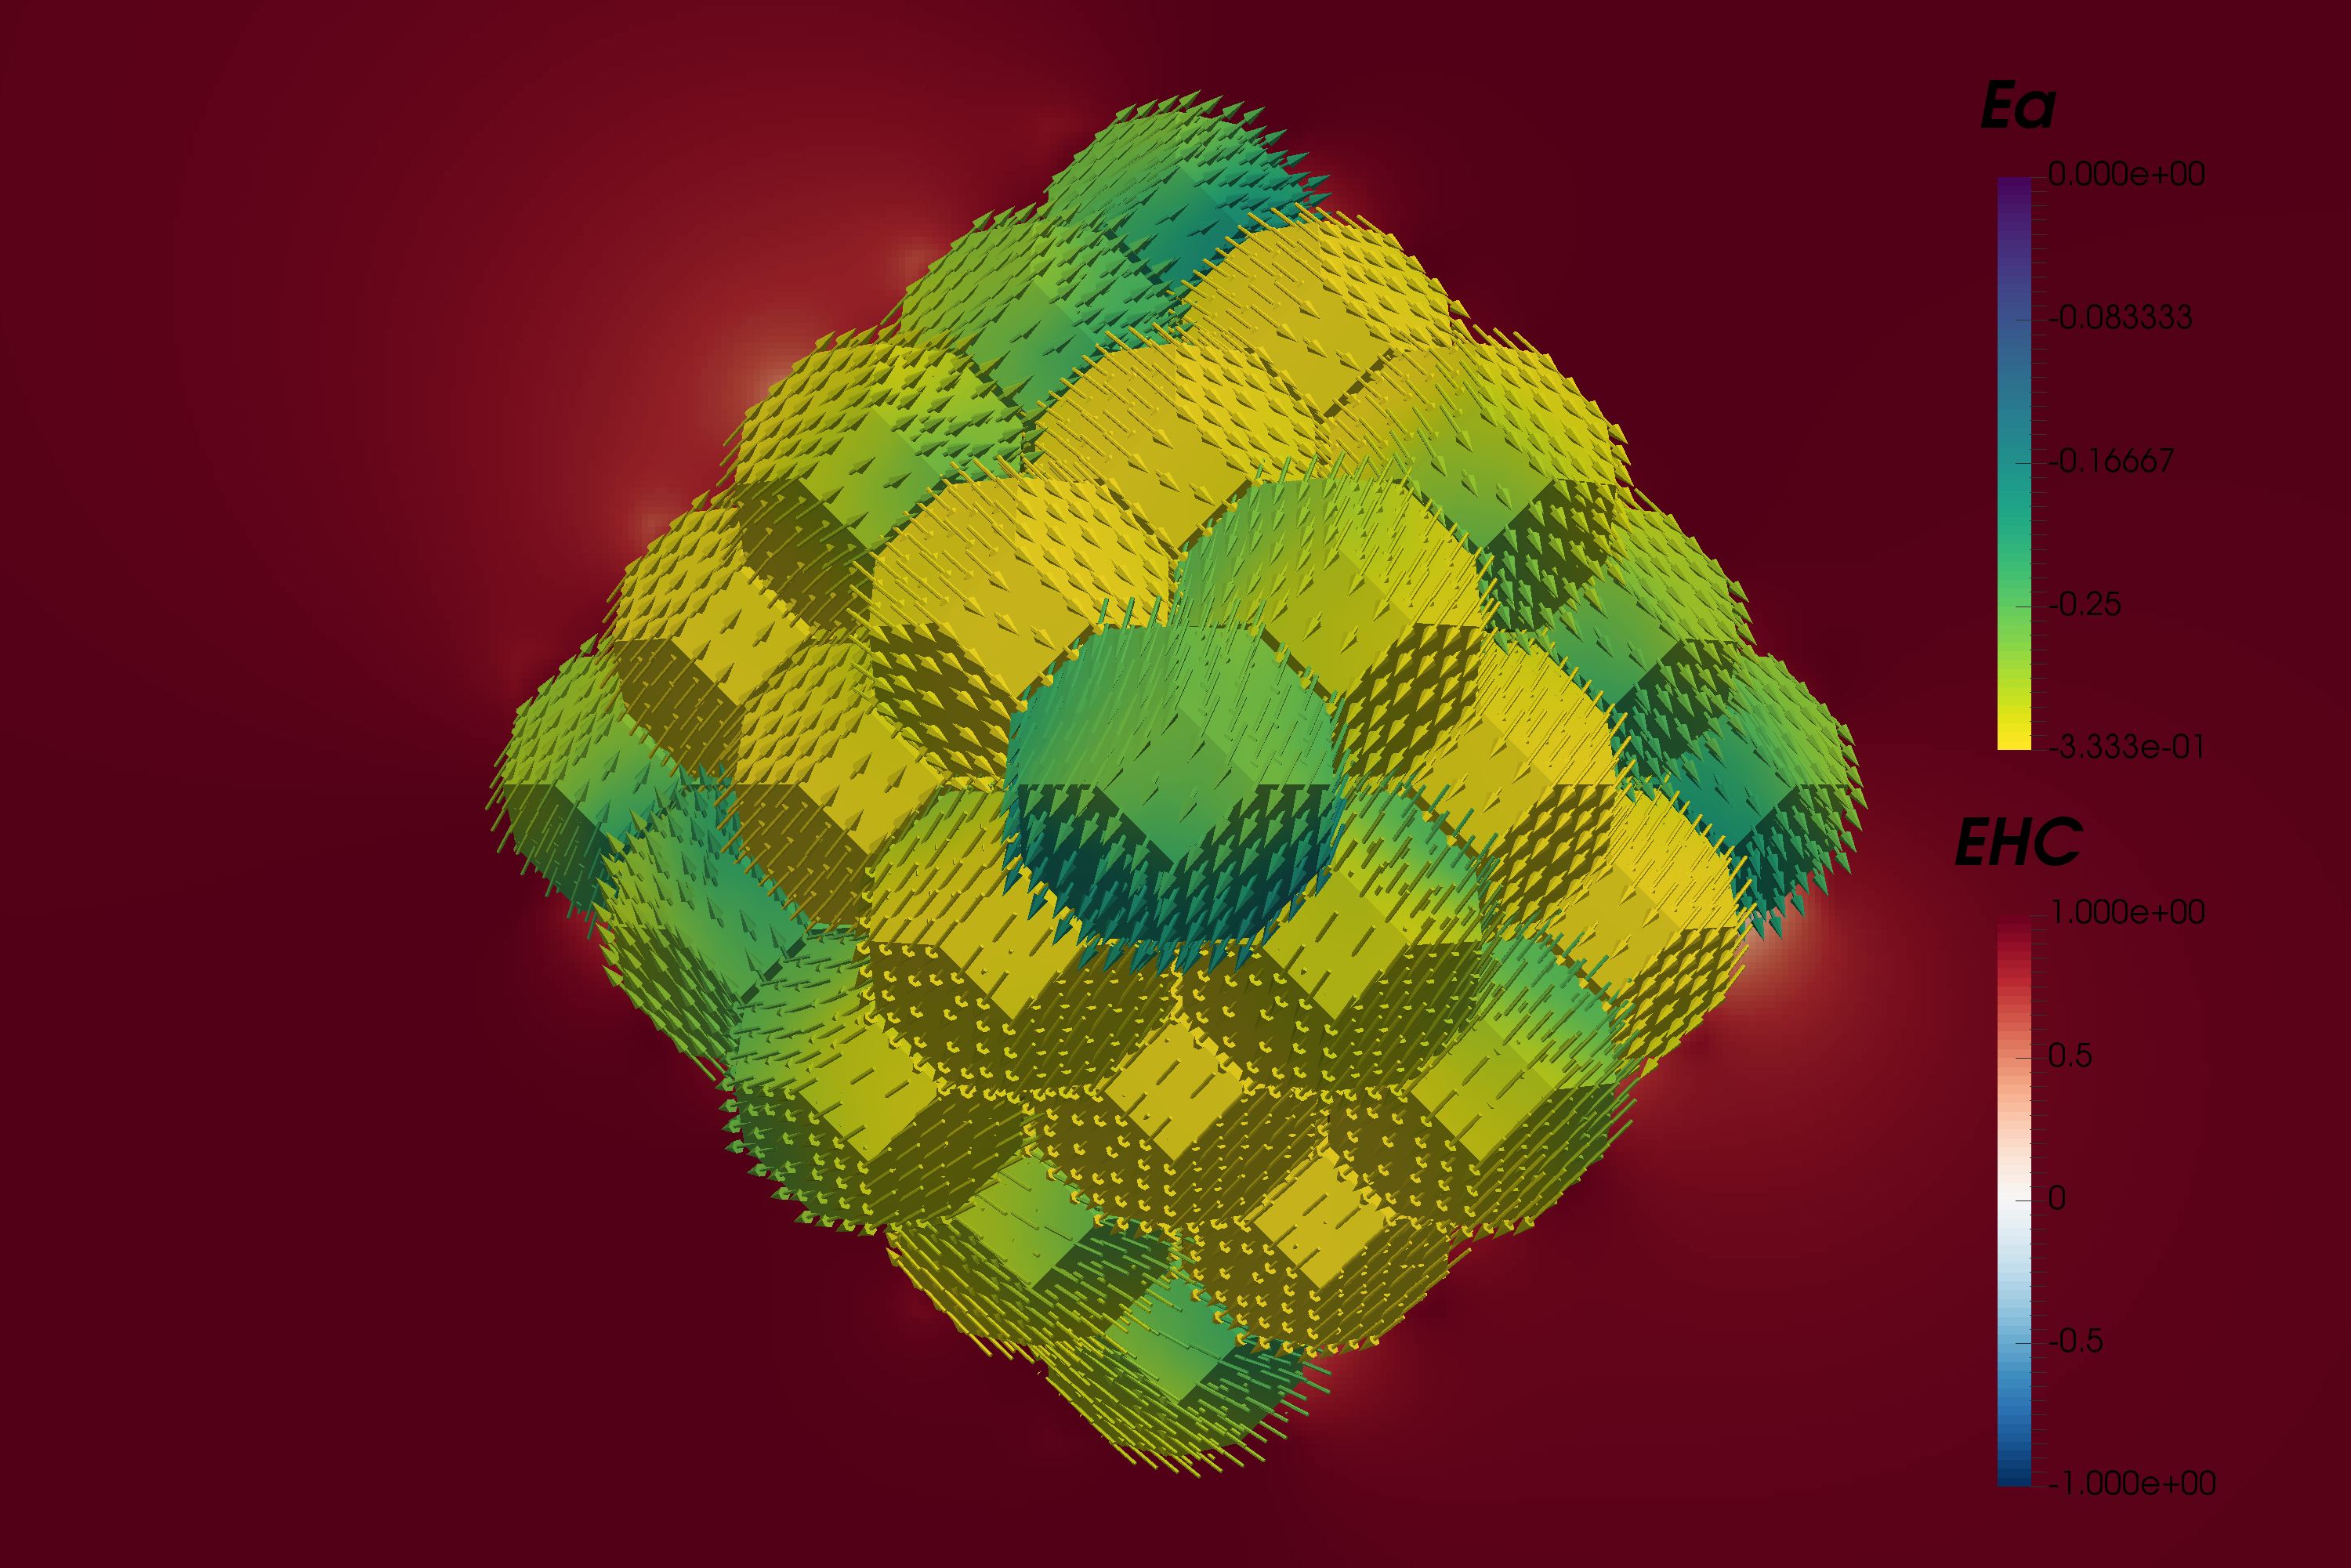
\includegraphics[width=\textwidth]{research-4/figs/fram_i16_f0_-z.png}
\caption[Remanent state when the field is along a hard axis (view from +Z)]{Remanent state when the field is along a hard axis (view from +Z).}
\label{FIG_21}
\end{figure}

\begin{figure}
\centering
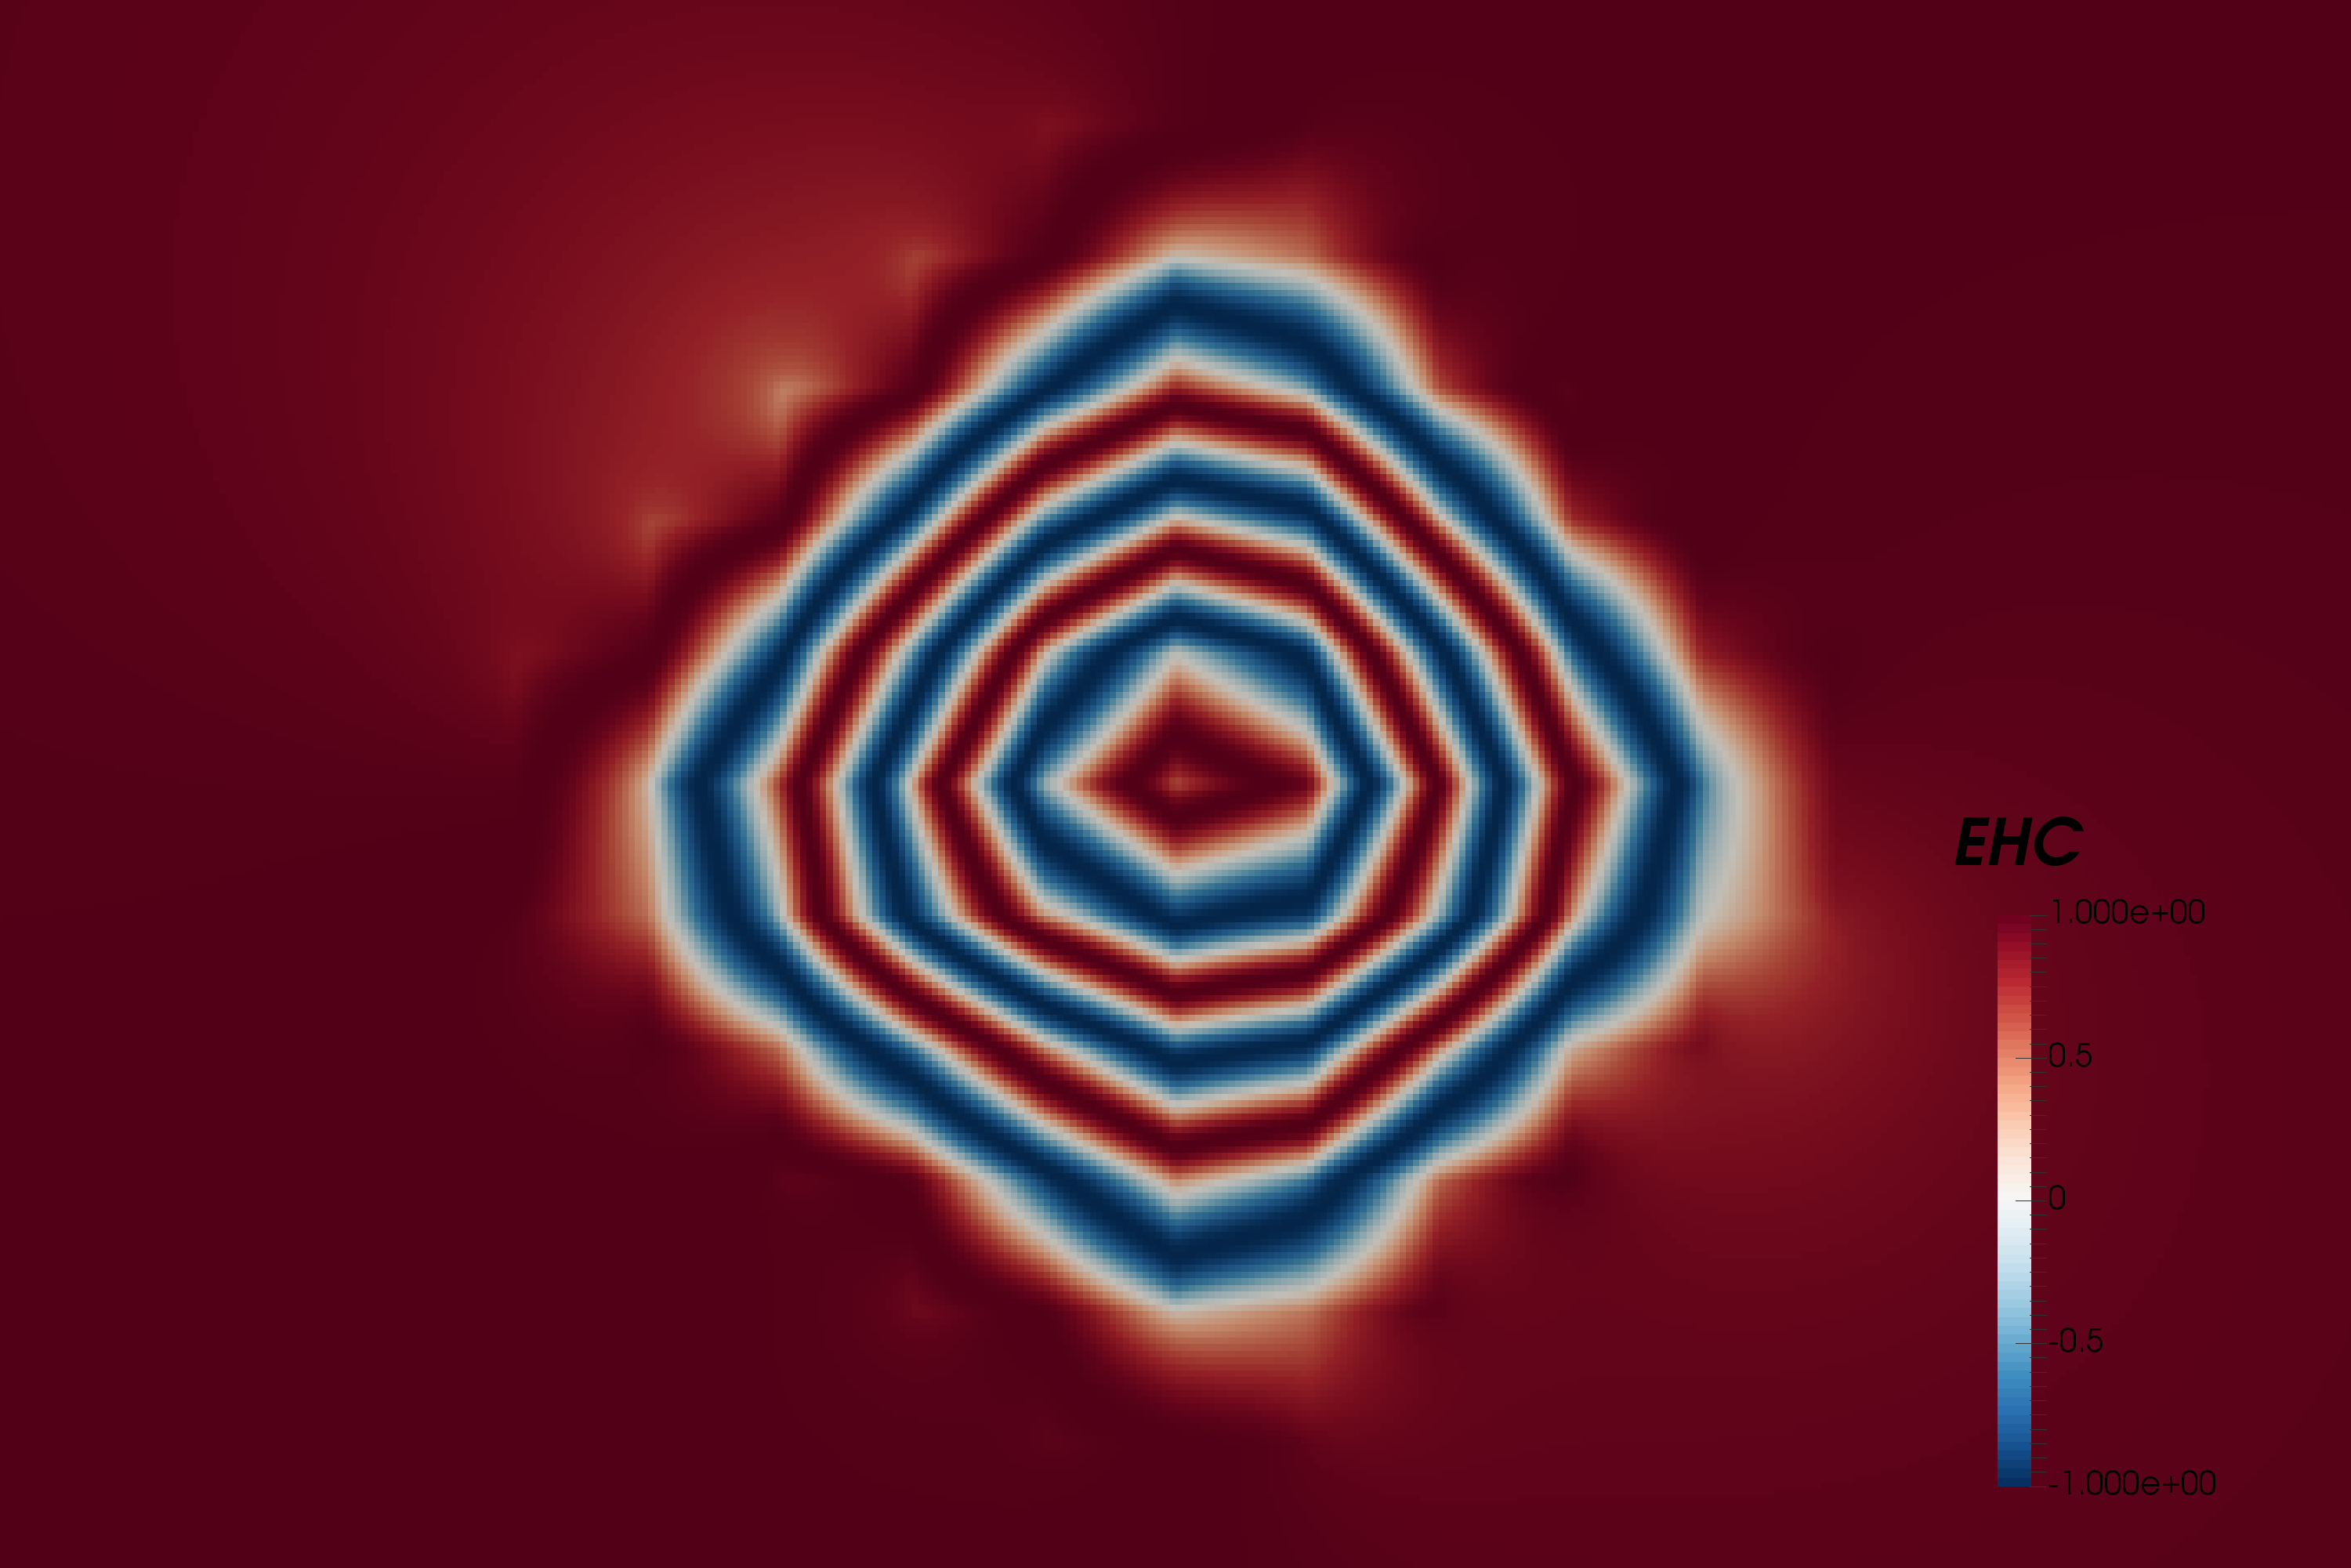
\includegraphics[width=\textwidth]{research-4/figs/fram_i16_f0_-z_EHC.png}
\caption[Electron holography map of the remanent state when the field is along a hard axis (view from +Z)]{Electron holography map of the remanent state when the field is along a hard axis (view from +Z).}
\label{FIG_22}
\end{figure}

\begin{figure}
\centering
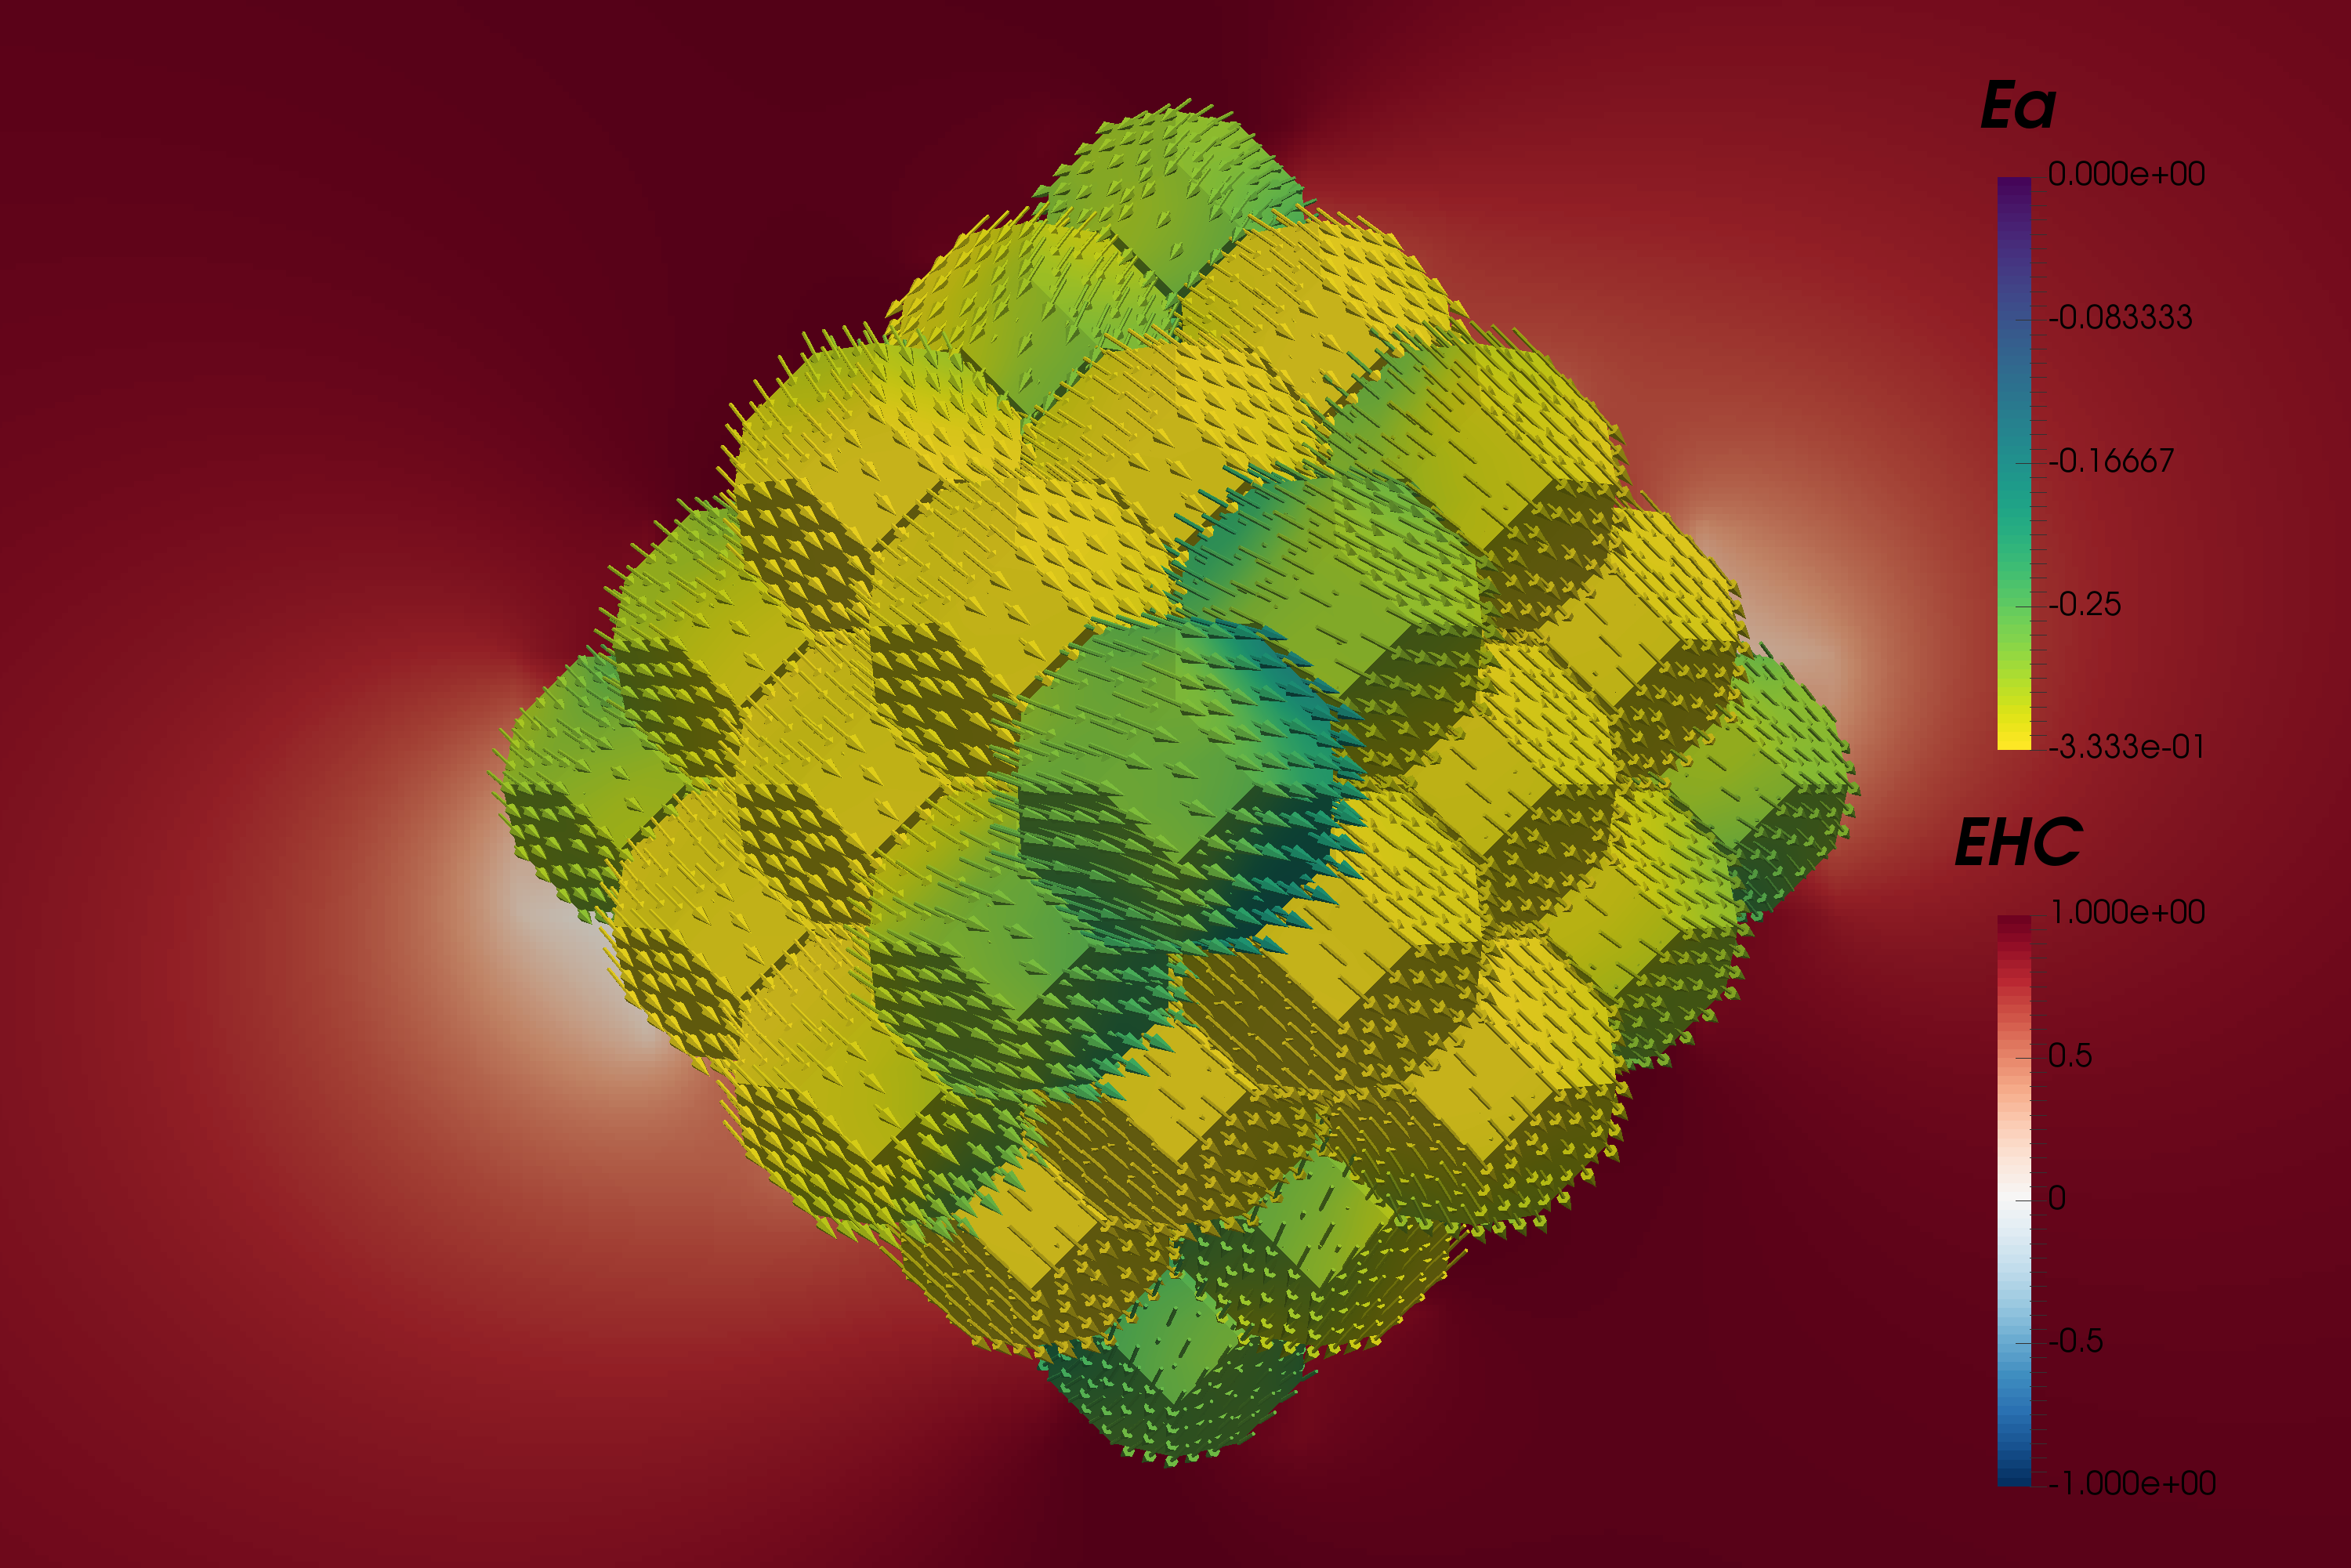
\includegraphics[width=\textwidth]{research-4/figs/fram_i16_f0_-y.png}
\caption[Remanent state when the field is along a hard axis (view from +Y)]{Remanent state when the field is along a hard axis (view from +Y).}
\label{FIG_23}
\end{figure}

\begin{figure}
\centering
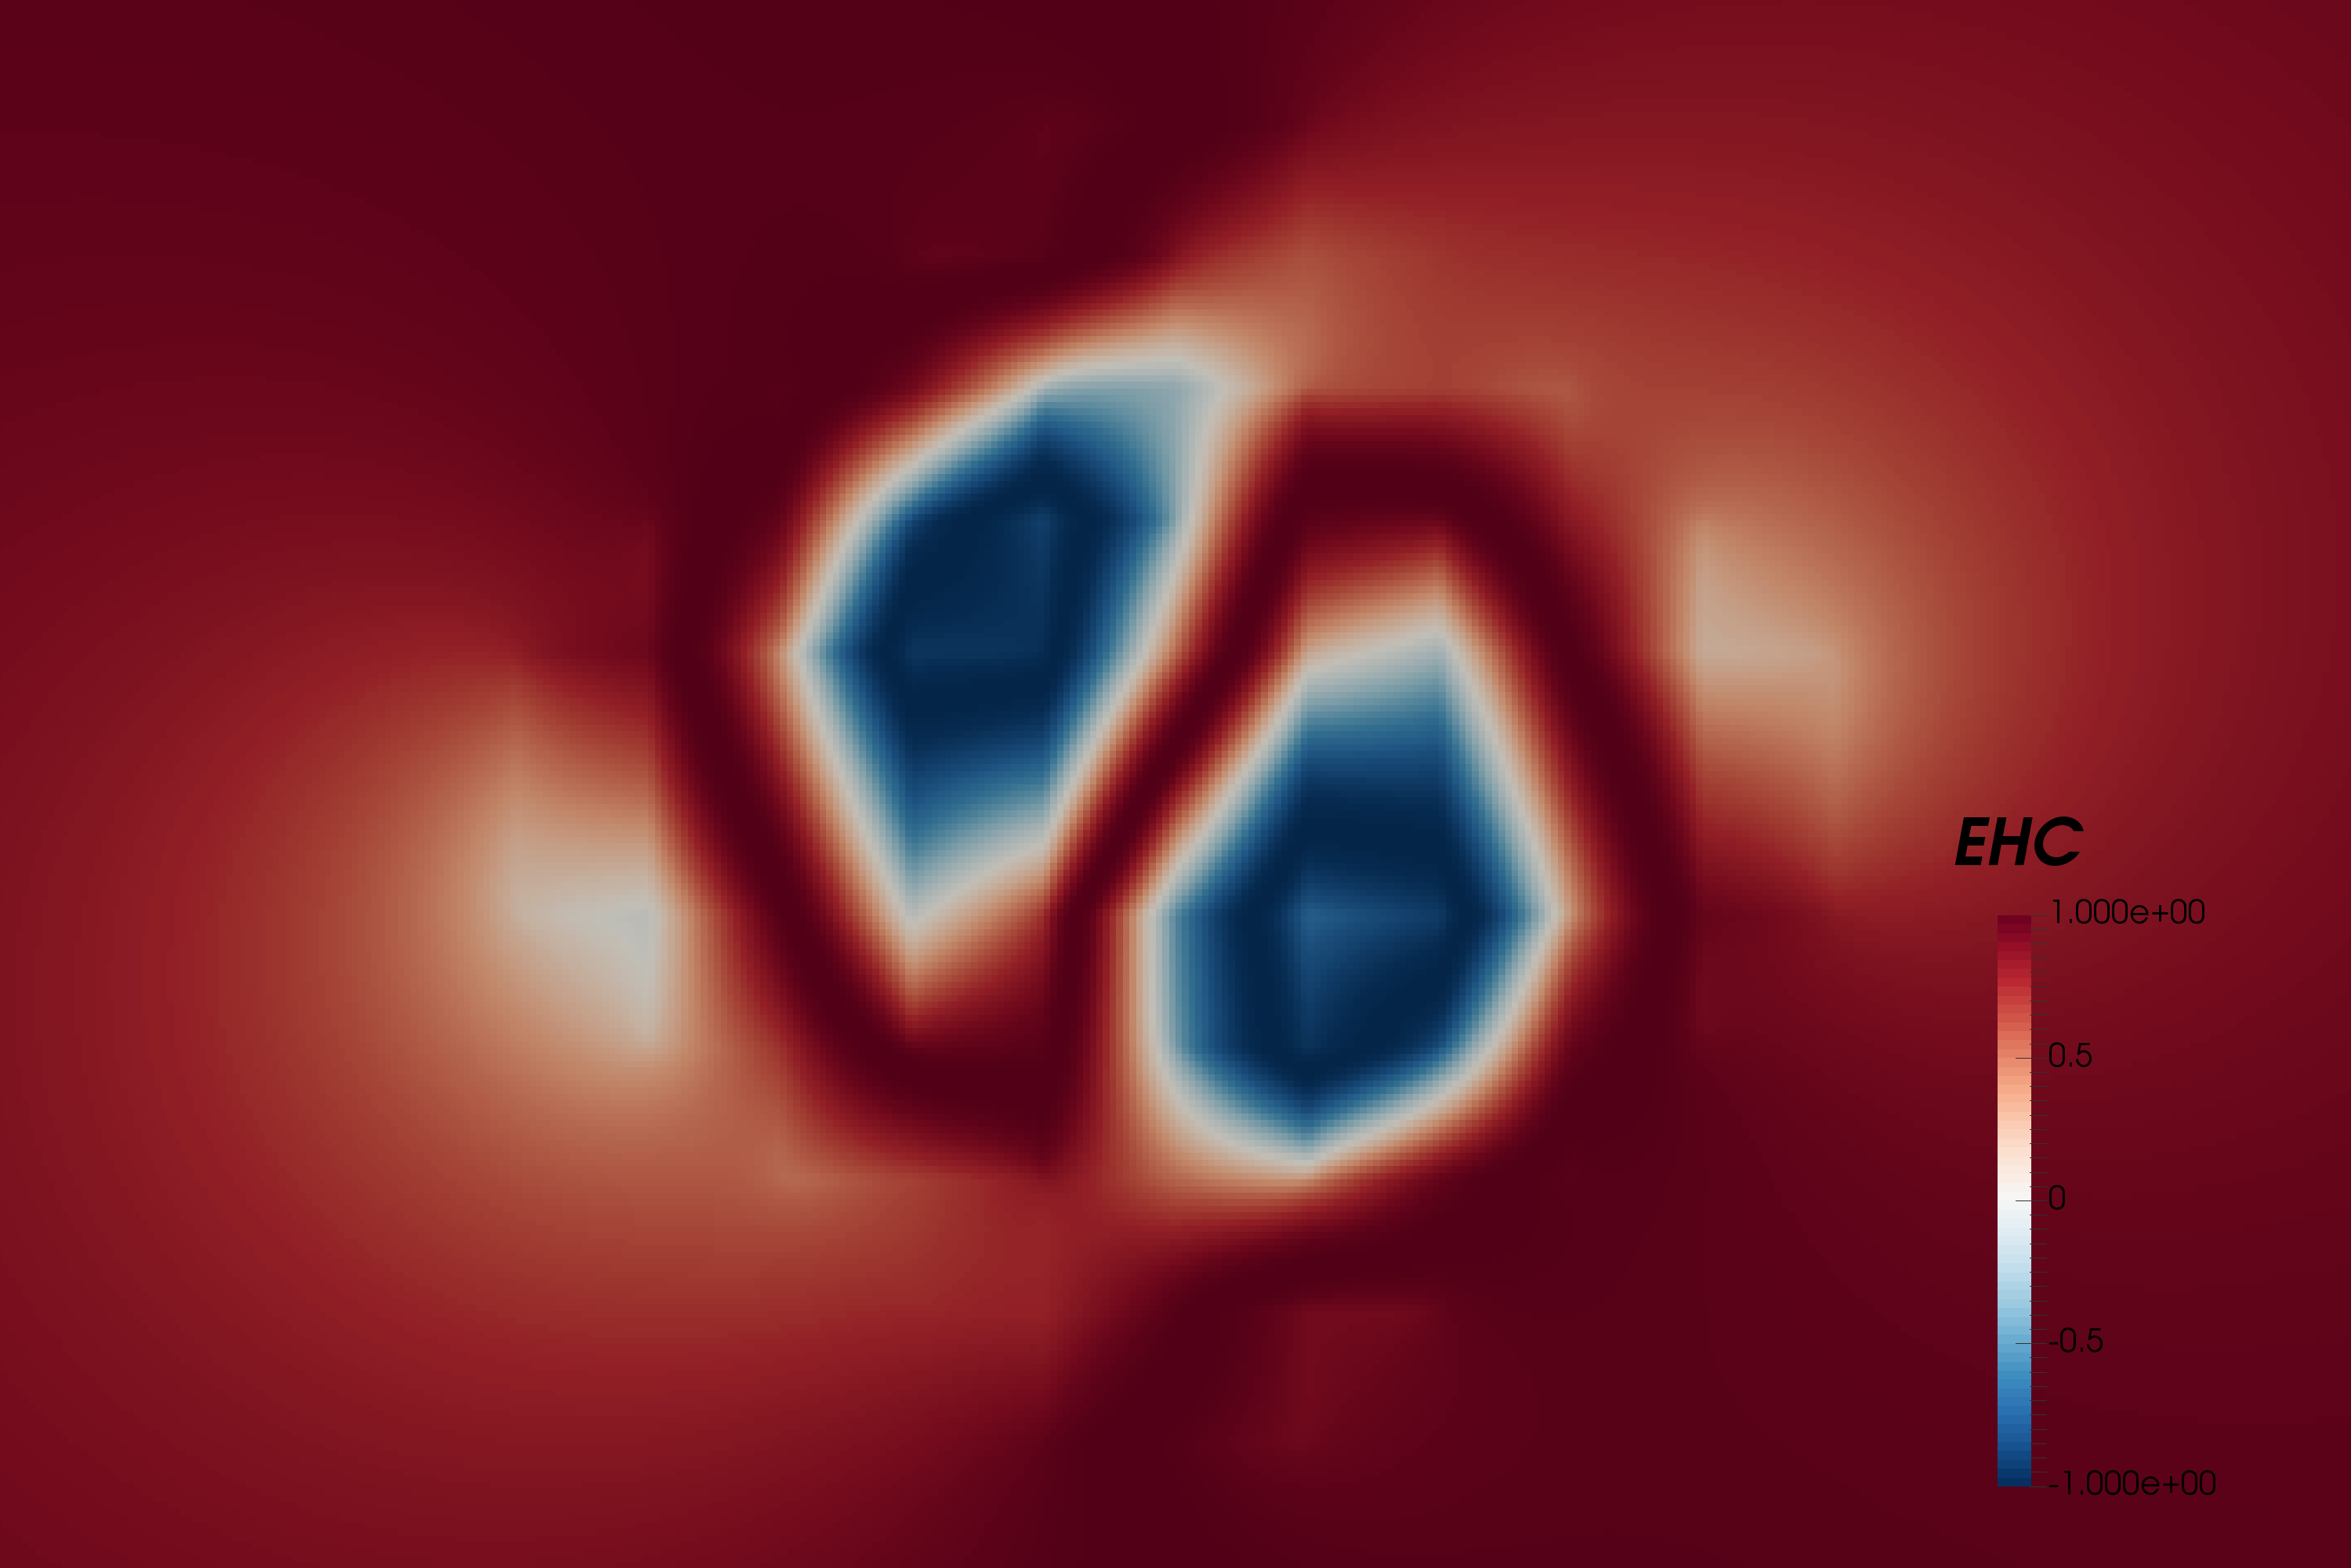
\includegraphics[width=\textwidth]{research-4/figs/fram_i16_f0_-y_EHC.png}
\caption[Electron holography map of the remanent state when the field is along a hard axis (view from +Y)]{Electron holography map of the remanent state when the field is along a hard axis (view from +Y).}
\label{FIG_24}
\end{figure}

\begin{figure}
\centering
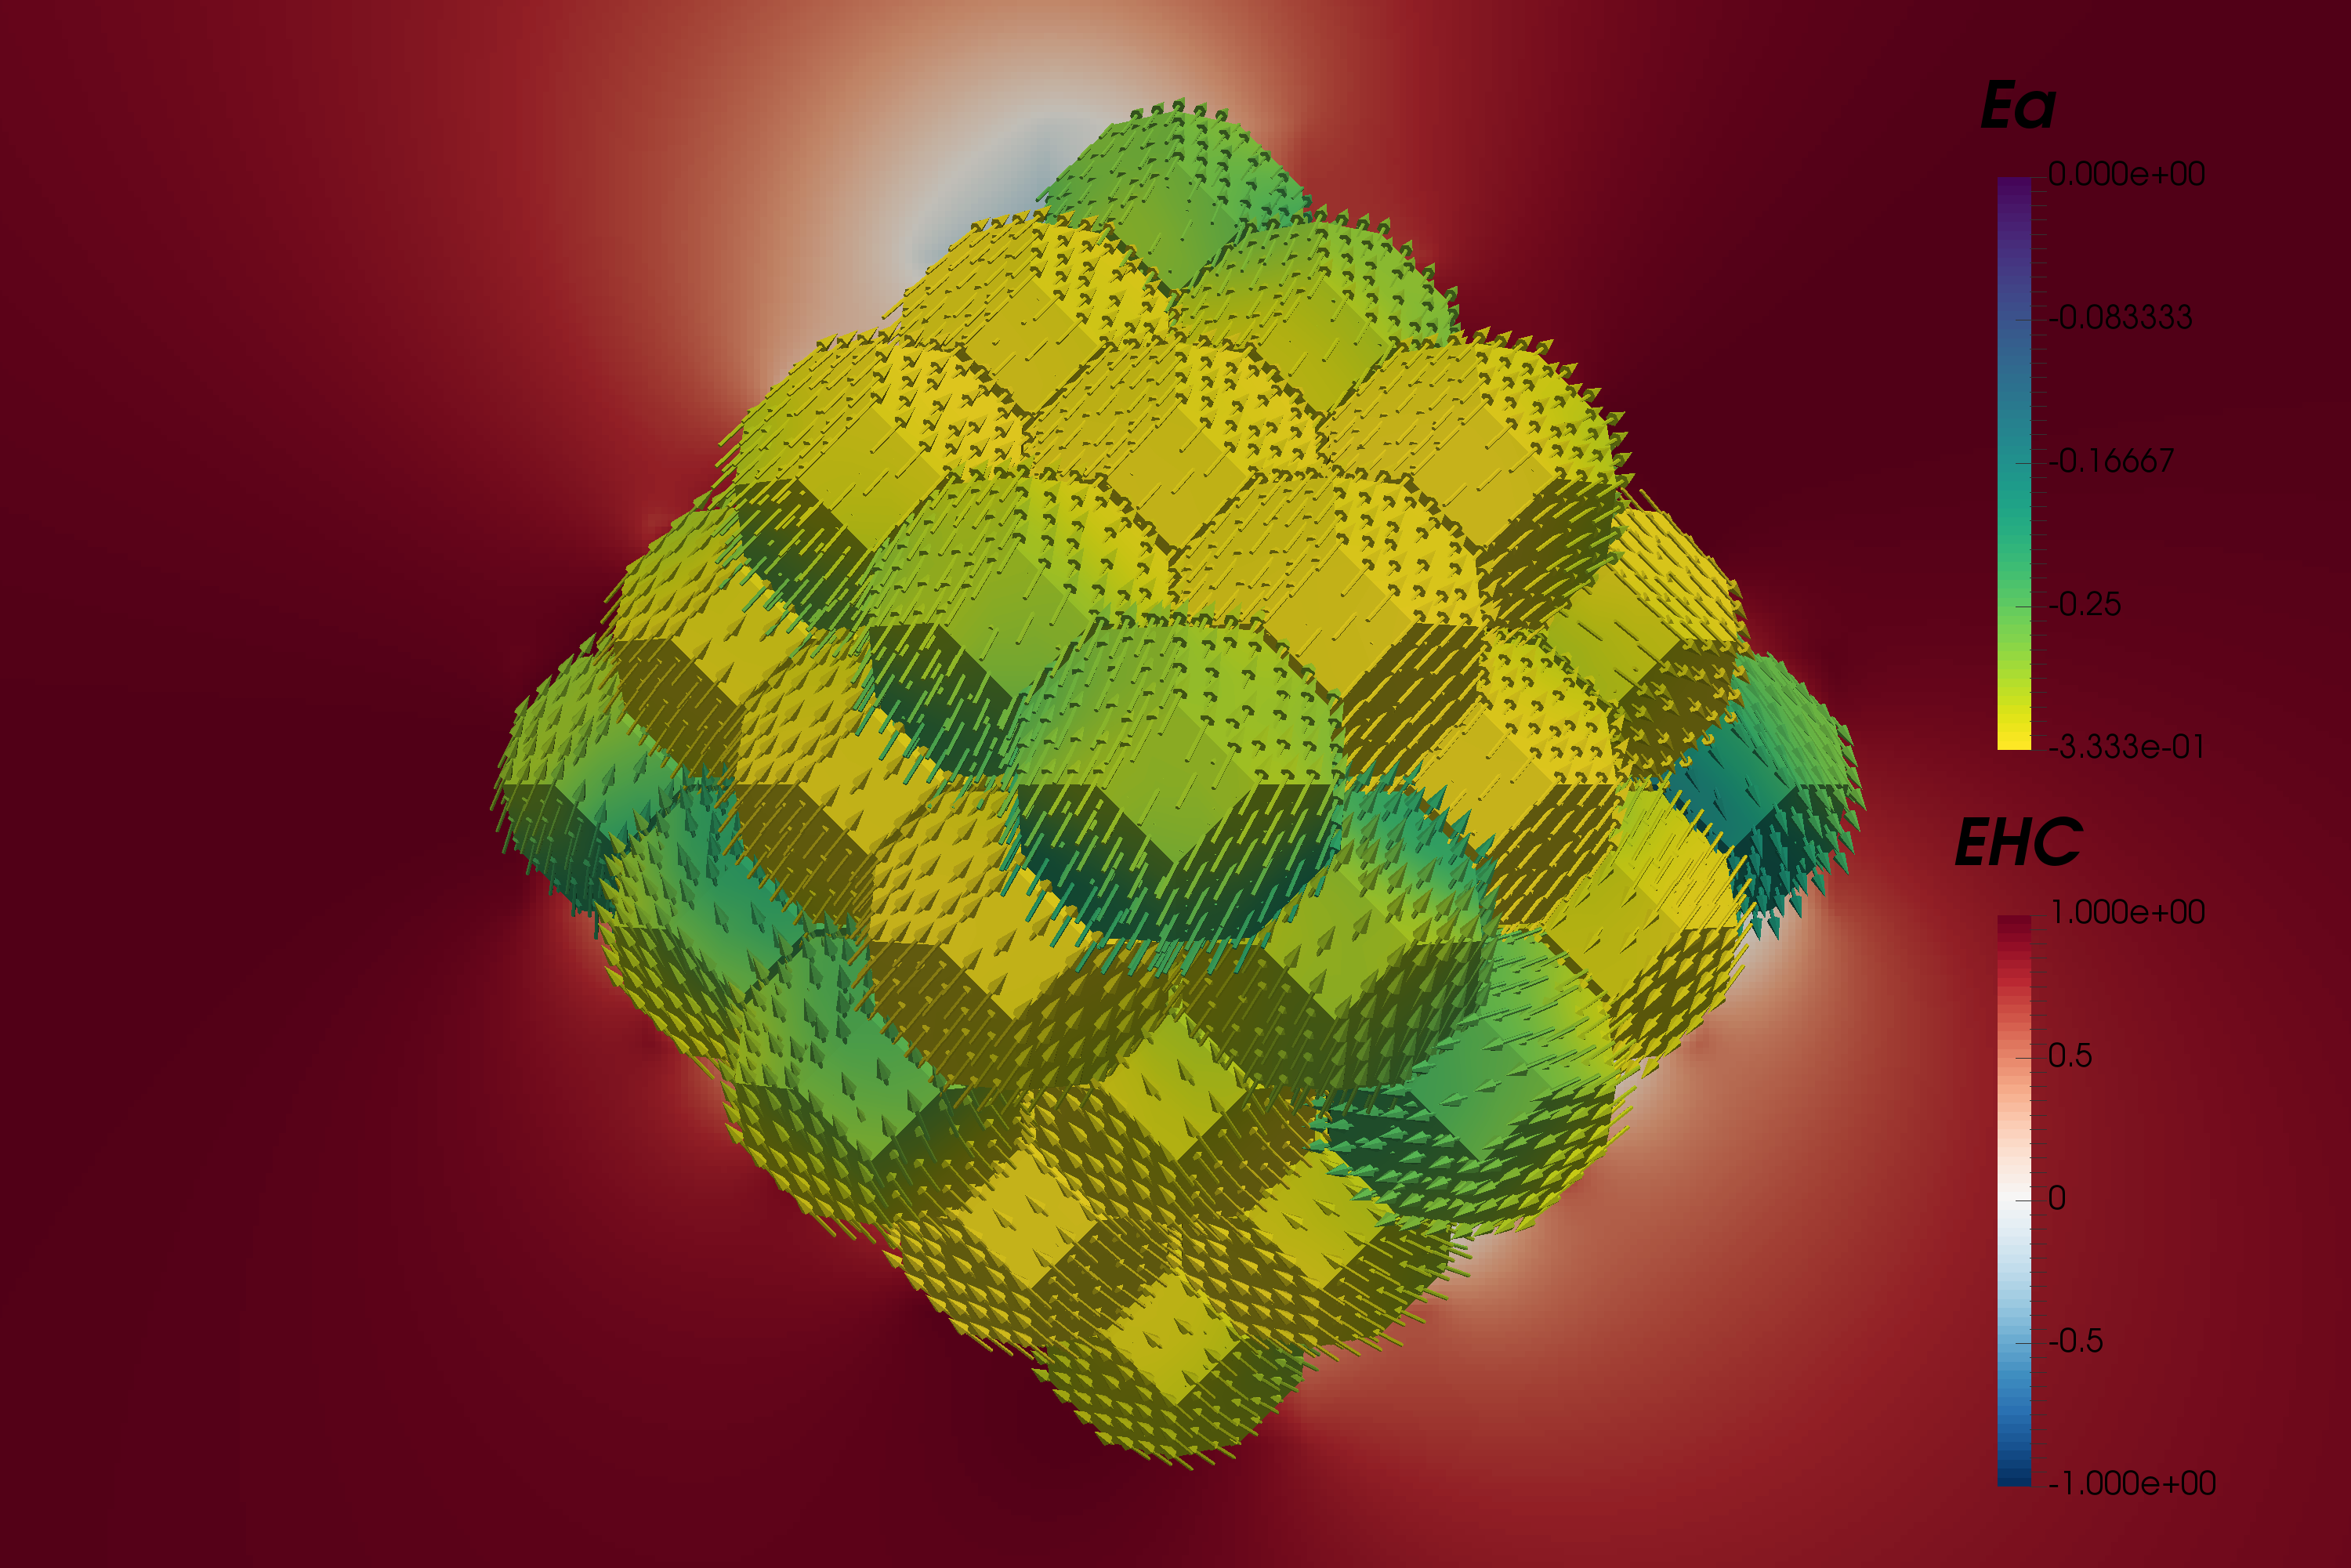
\includegraphics[width=\textwidth]{research-4/figs/fram_i16_f0_-x.png}
\caption[Remanent state when the field is along a hard axis (view from +X)]{Remanent state when the field is along a hard axis (view from +X).}
\label{FIG_25}
\end{figure}

\begin{figure}
\centering
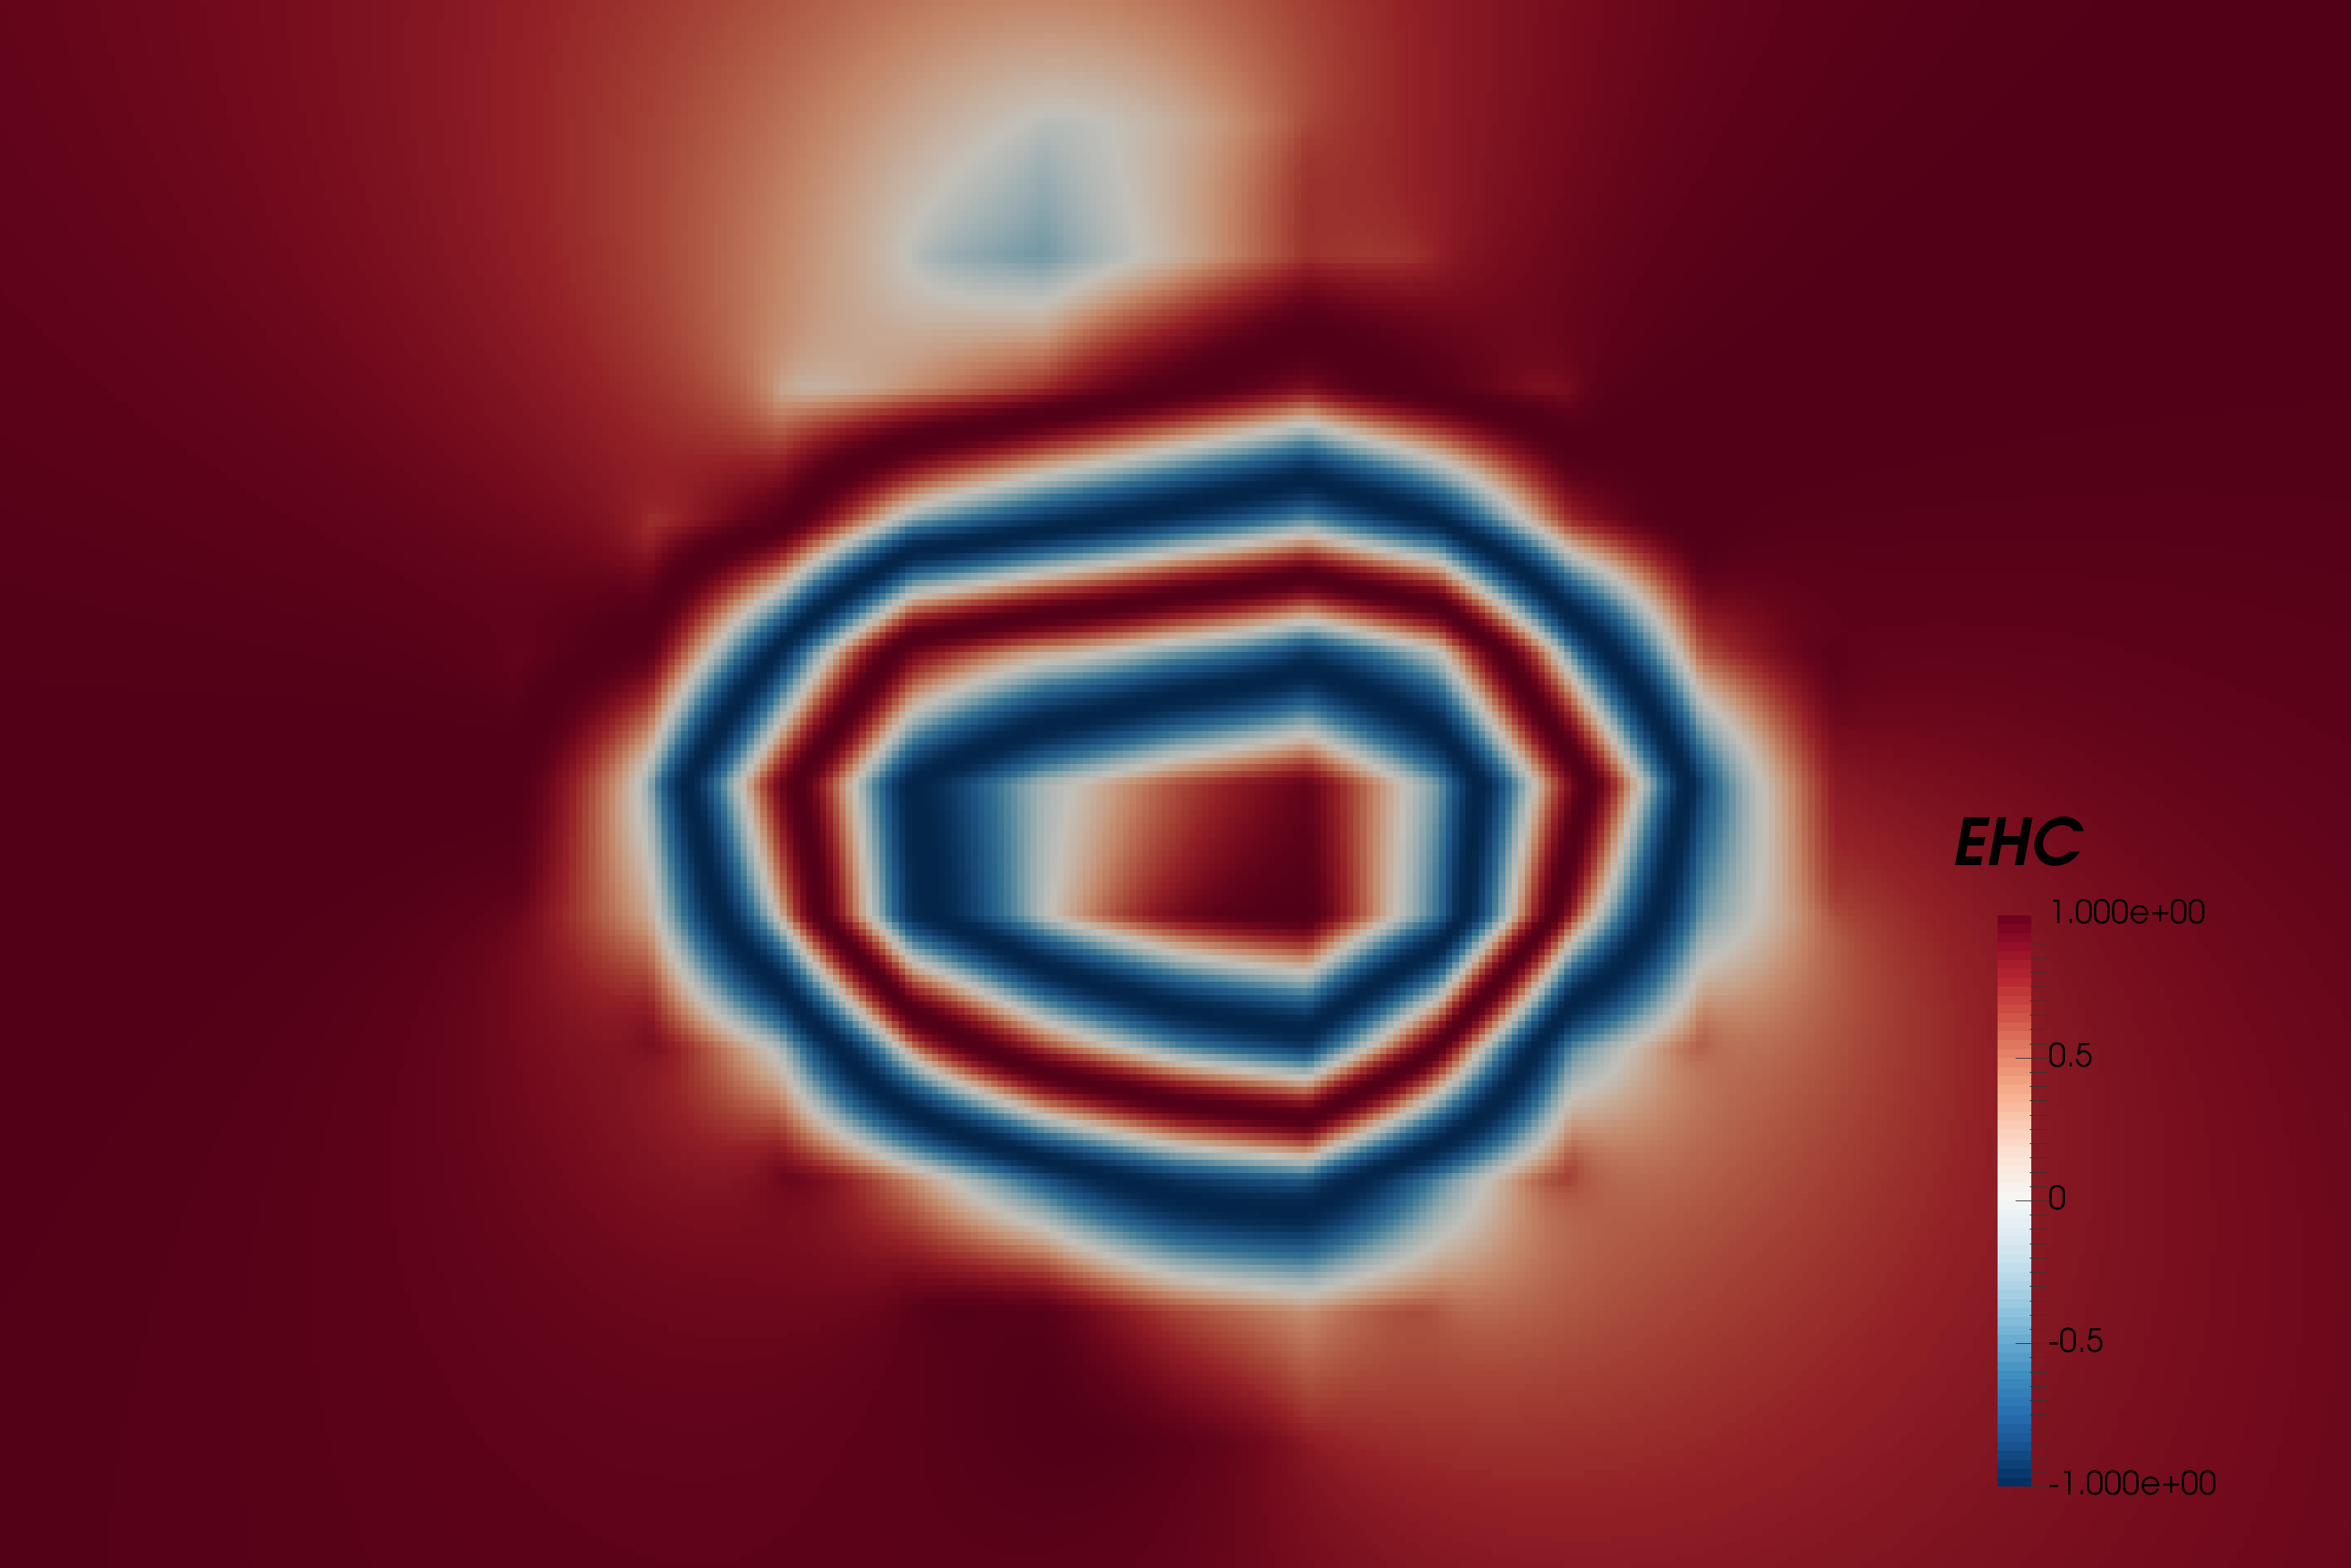
\includegraphics[width=\textwidth]{research-4/figs/fram_i16_f0_-x_EHC.png}
\caption[Electron holography map of the remanent state when the field is along a hard axis (view from +X)]{Electron holography map of the remanent state when the field is along a hard axis (view from +X).}
\label{FIG_26}
\end{figure}

\subsection{Hysteresis and remanent states of larger particle framboids.}
I calculated the hysteresis curves of smaller (less particles) framboids with 76$\nm$ particles (which are strictly SV when isolated) for the field directions I showed individual FORC diagrams for earlier in this chapter. I want to show here some of them and the remanent states with electron holography images. I had no time to finish those plots. The particles are not SD anymore, although the innermost particle does seem to remain SD during hysteresis.\par

\section{Discussion}
Discussion section...\par

\section{Conclusions}
Conclusion section...\par

%----------------------------------
\renewcommand\bibname{{References}}
\bibliographystyle{elsarticle-harv}
\bibliography{references}

